\section{Results}


\subsection{Hypothese 1: Themen der Bundestagsreden}

{\bfseries Methodologie Hypothese 1a \& 1b:} Zur Überprüfung der Hypothesen wurde eine Stichprobe aus den Plenarprotokollen gezogen, die anschließend von Hand kodiert wurde. Für die Vergleichbarkeit der Ergebnisse besteht die Stichprobe aus jeweils 59 Reden, die in dem ersten Jahr nach Beginn der Legislaturperiode gehalten wurden. Die Stichprobe wurde zweistufig gezogen: Aus jedem Zeitraum wurden 59 Plenarprotokolle ausgewählt, das sind 2017 alle Protokolle, 2013 59 aus 60 und 2009 59 aus 67. Aus jeder der 59 Plenarprotokollen wurde jeweils eine Rede zufällig ausgewählt und den Kodierern zufällig zugeteilt. Kodiert wurde der thematische Inhalt von der Rede und der thematische Inhalt vom dazugehörigen Tagesordnungspunkt. Zusätzlich wurden 10 Reden pro Kodierer auf zwei weitere Kodierer aufgeteilt, und die Interkoder-Reliabilität getestet.\\

\subsubsection{Reliabilität der Stichprobe} 
Die Variable v101 steht für Finanzen und ihre niedrige Reliabilität lässt sich damit erklären, dass Finanzen ... Die Reliabilität liegt mit 0.57 außerhalb/innerhalb von ...  
\begin{table}[H]
	\centering
	\begin{longtable}{rrrrr}
		\hline
		Variable & Mehmet und Nils & Mehmet und Vivian & Vivian und Nils & Durchschnitt \\ 
		\hline \hline
		v105 & / & 0.94 & / & / \\ 
		v300 & 0.93 & 0.75 & 1.00 & 0.83 \\ 
		v219 & / & / & 0.93 & / \\ 
		v206 & 0.93 & 0.94 & 1.00 & 0.96 \\ 
		v205 & 0.79 & 0.88 & 0.93 & 0.89 \\ 
		v204 & / & / & 1.00 & / \\ 
		v203 & 0.93 & 0.94 & 0.71 & 0.86 \\ 
		v202 & 0.79 & 0.75 & 0.93 & 0.81 \\ 
		v201 & 0.86 & 0.81 & 0.93 & 0.85 \\ 
		v119 & 0.93 & 0.94 & 0.86 & 0.91 \\ 
		v116 & 0.86 & 1.00 & 0.79 & 0.93 \\ 
		v115 & 1.00 & 1.00 & 1.00 & 1.00 \\ 
		v114 & 0.86 & 0.81 & 0.86 & 0.83 \\ 
		v113 & 0.93 & 0.81 & 0.86 & 0.83 \\ 
		v112 & 1.00 & 0.94 & 0.79 & 0.89 \\ 
		v111 & 1.00 & 0.88 & 0.79 & 0.85 \\ 
		v110 & 0.86 & 0.88 & 0.93 & 0.89 \\ 
		v109 & 0.86 & 0.88 & 1.00 & 0.92 \\ 
		v108 & 1.00 & 1.00 & 1.00 & 1.00 \\ 
		v107 & 0.79 & 0.69 & 0.86 & 0.74 \\ 
		v106 & 0.93 & 1.00 & 1.00 & 1.00 \\ 
		v104 & 0.93 & 0.94 & 1.00 & 0.96 \\ 
		v103 & 0.79 & 0.88 & 0.86 & 0.87 \\ 
		v102 & 0.79 & 0.62 & 0.71 & 0.65 \\ 
		v101 & 0.57 & 0.50 & 0.71 & 0.57 \\ 
		\hline
	\end{longtable}
\end{table}



\subsubsection{Hypothese 1a: Wenige Themen dominieren}
\begin{figure} [h]
	\subfigure[2009]{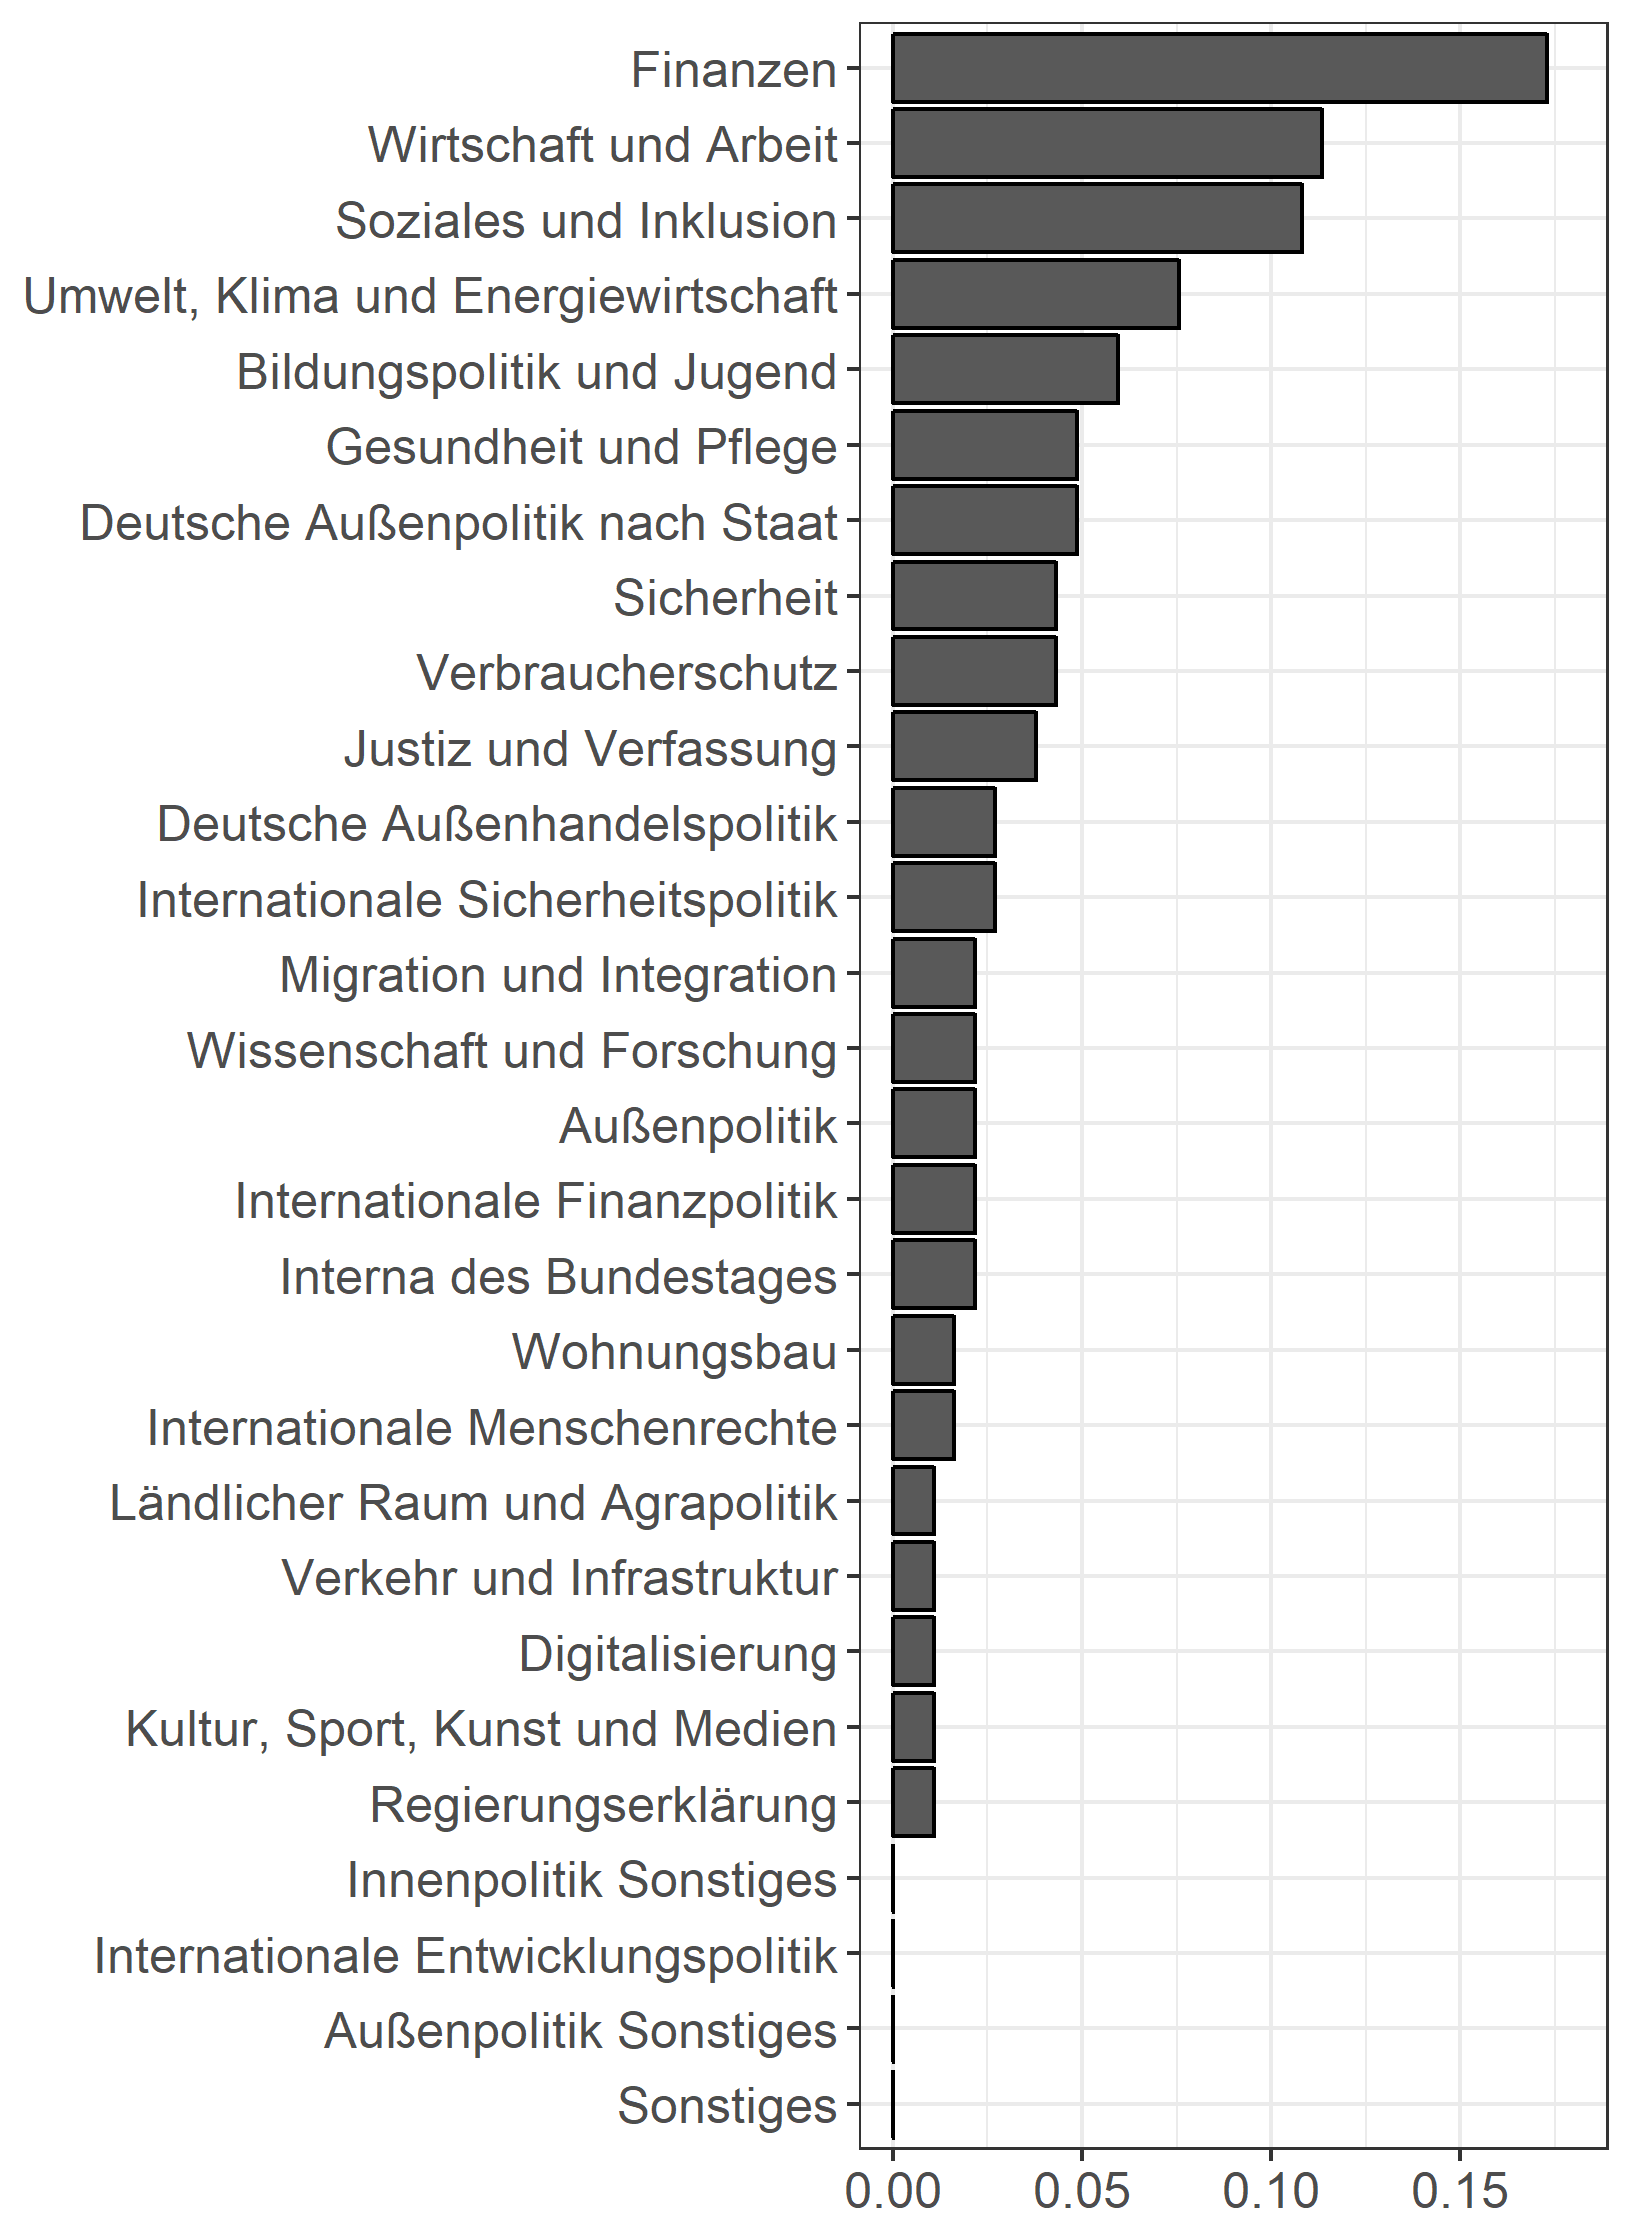
\includegraphics[width=0.29\textwidth]{Grafiken/Inhalt09.png}}
	\subfigure[2013]{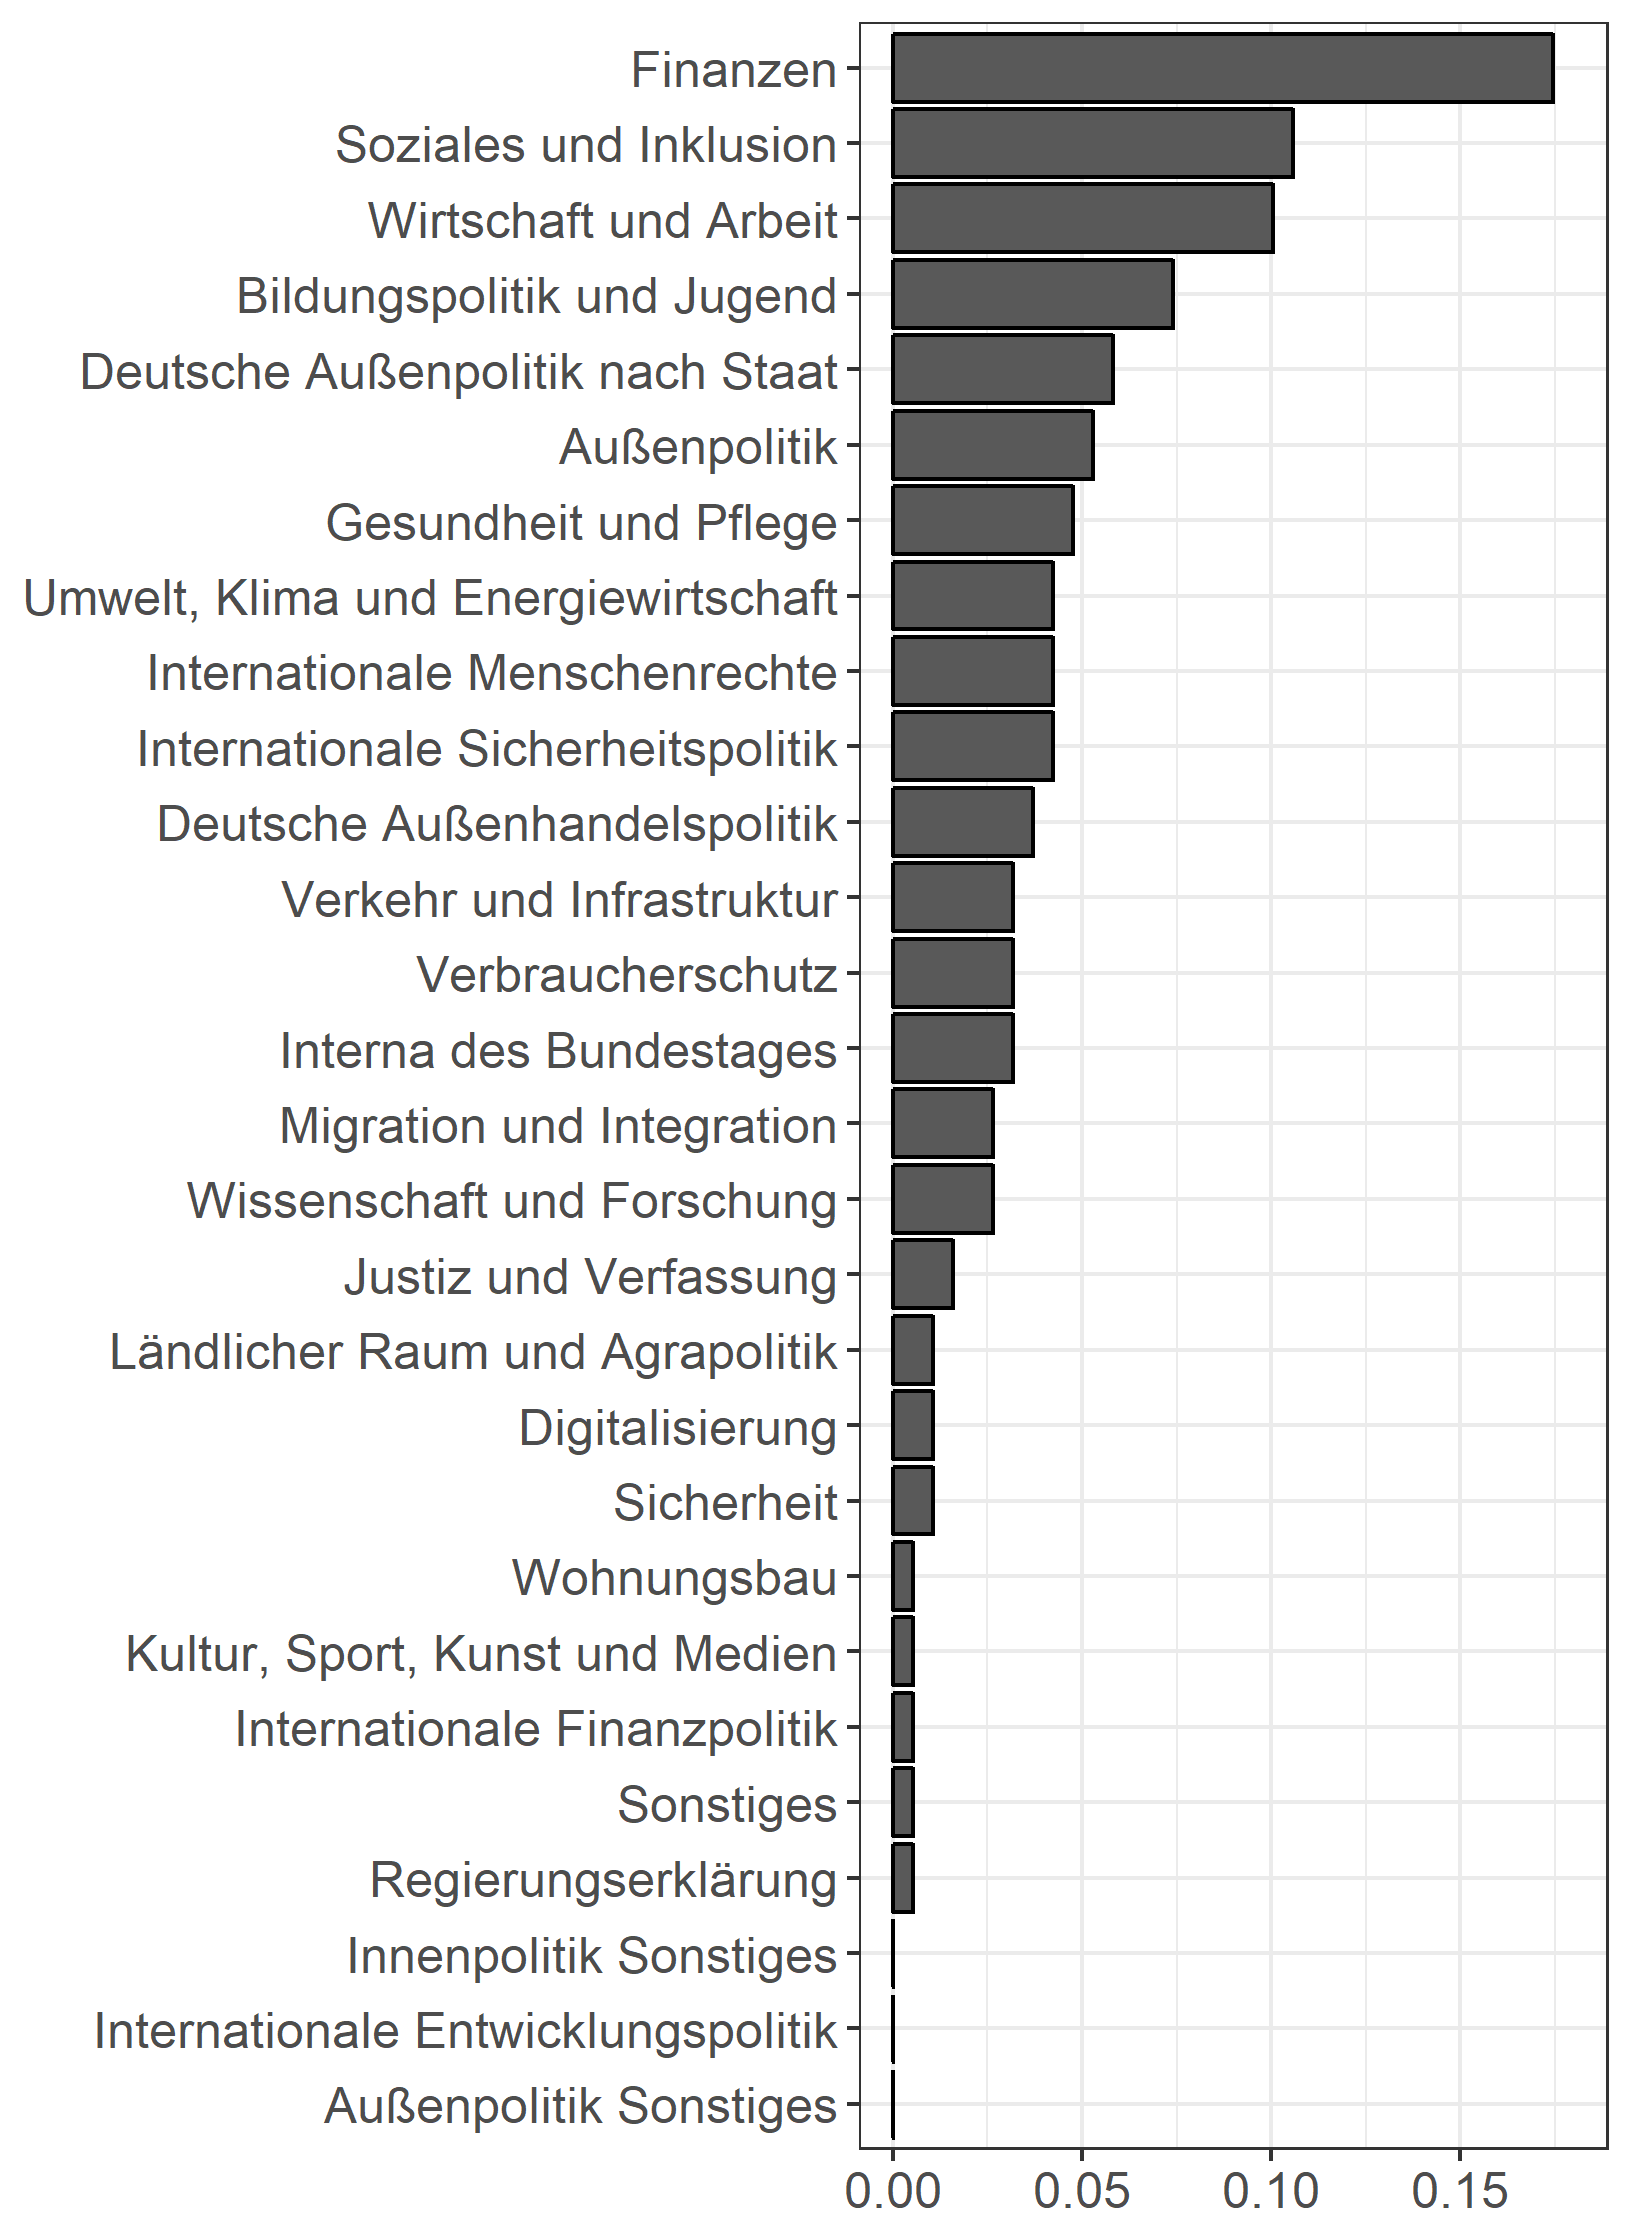
\includegraphics[width=0.29\textwidth]{Grafiken/Inhalt13.png}}
	\subfigure[2017]{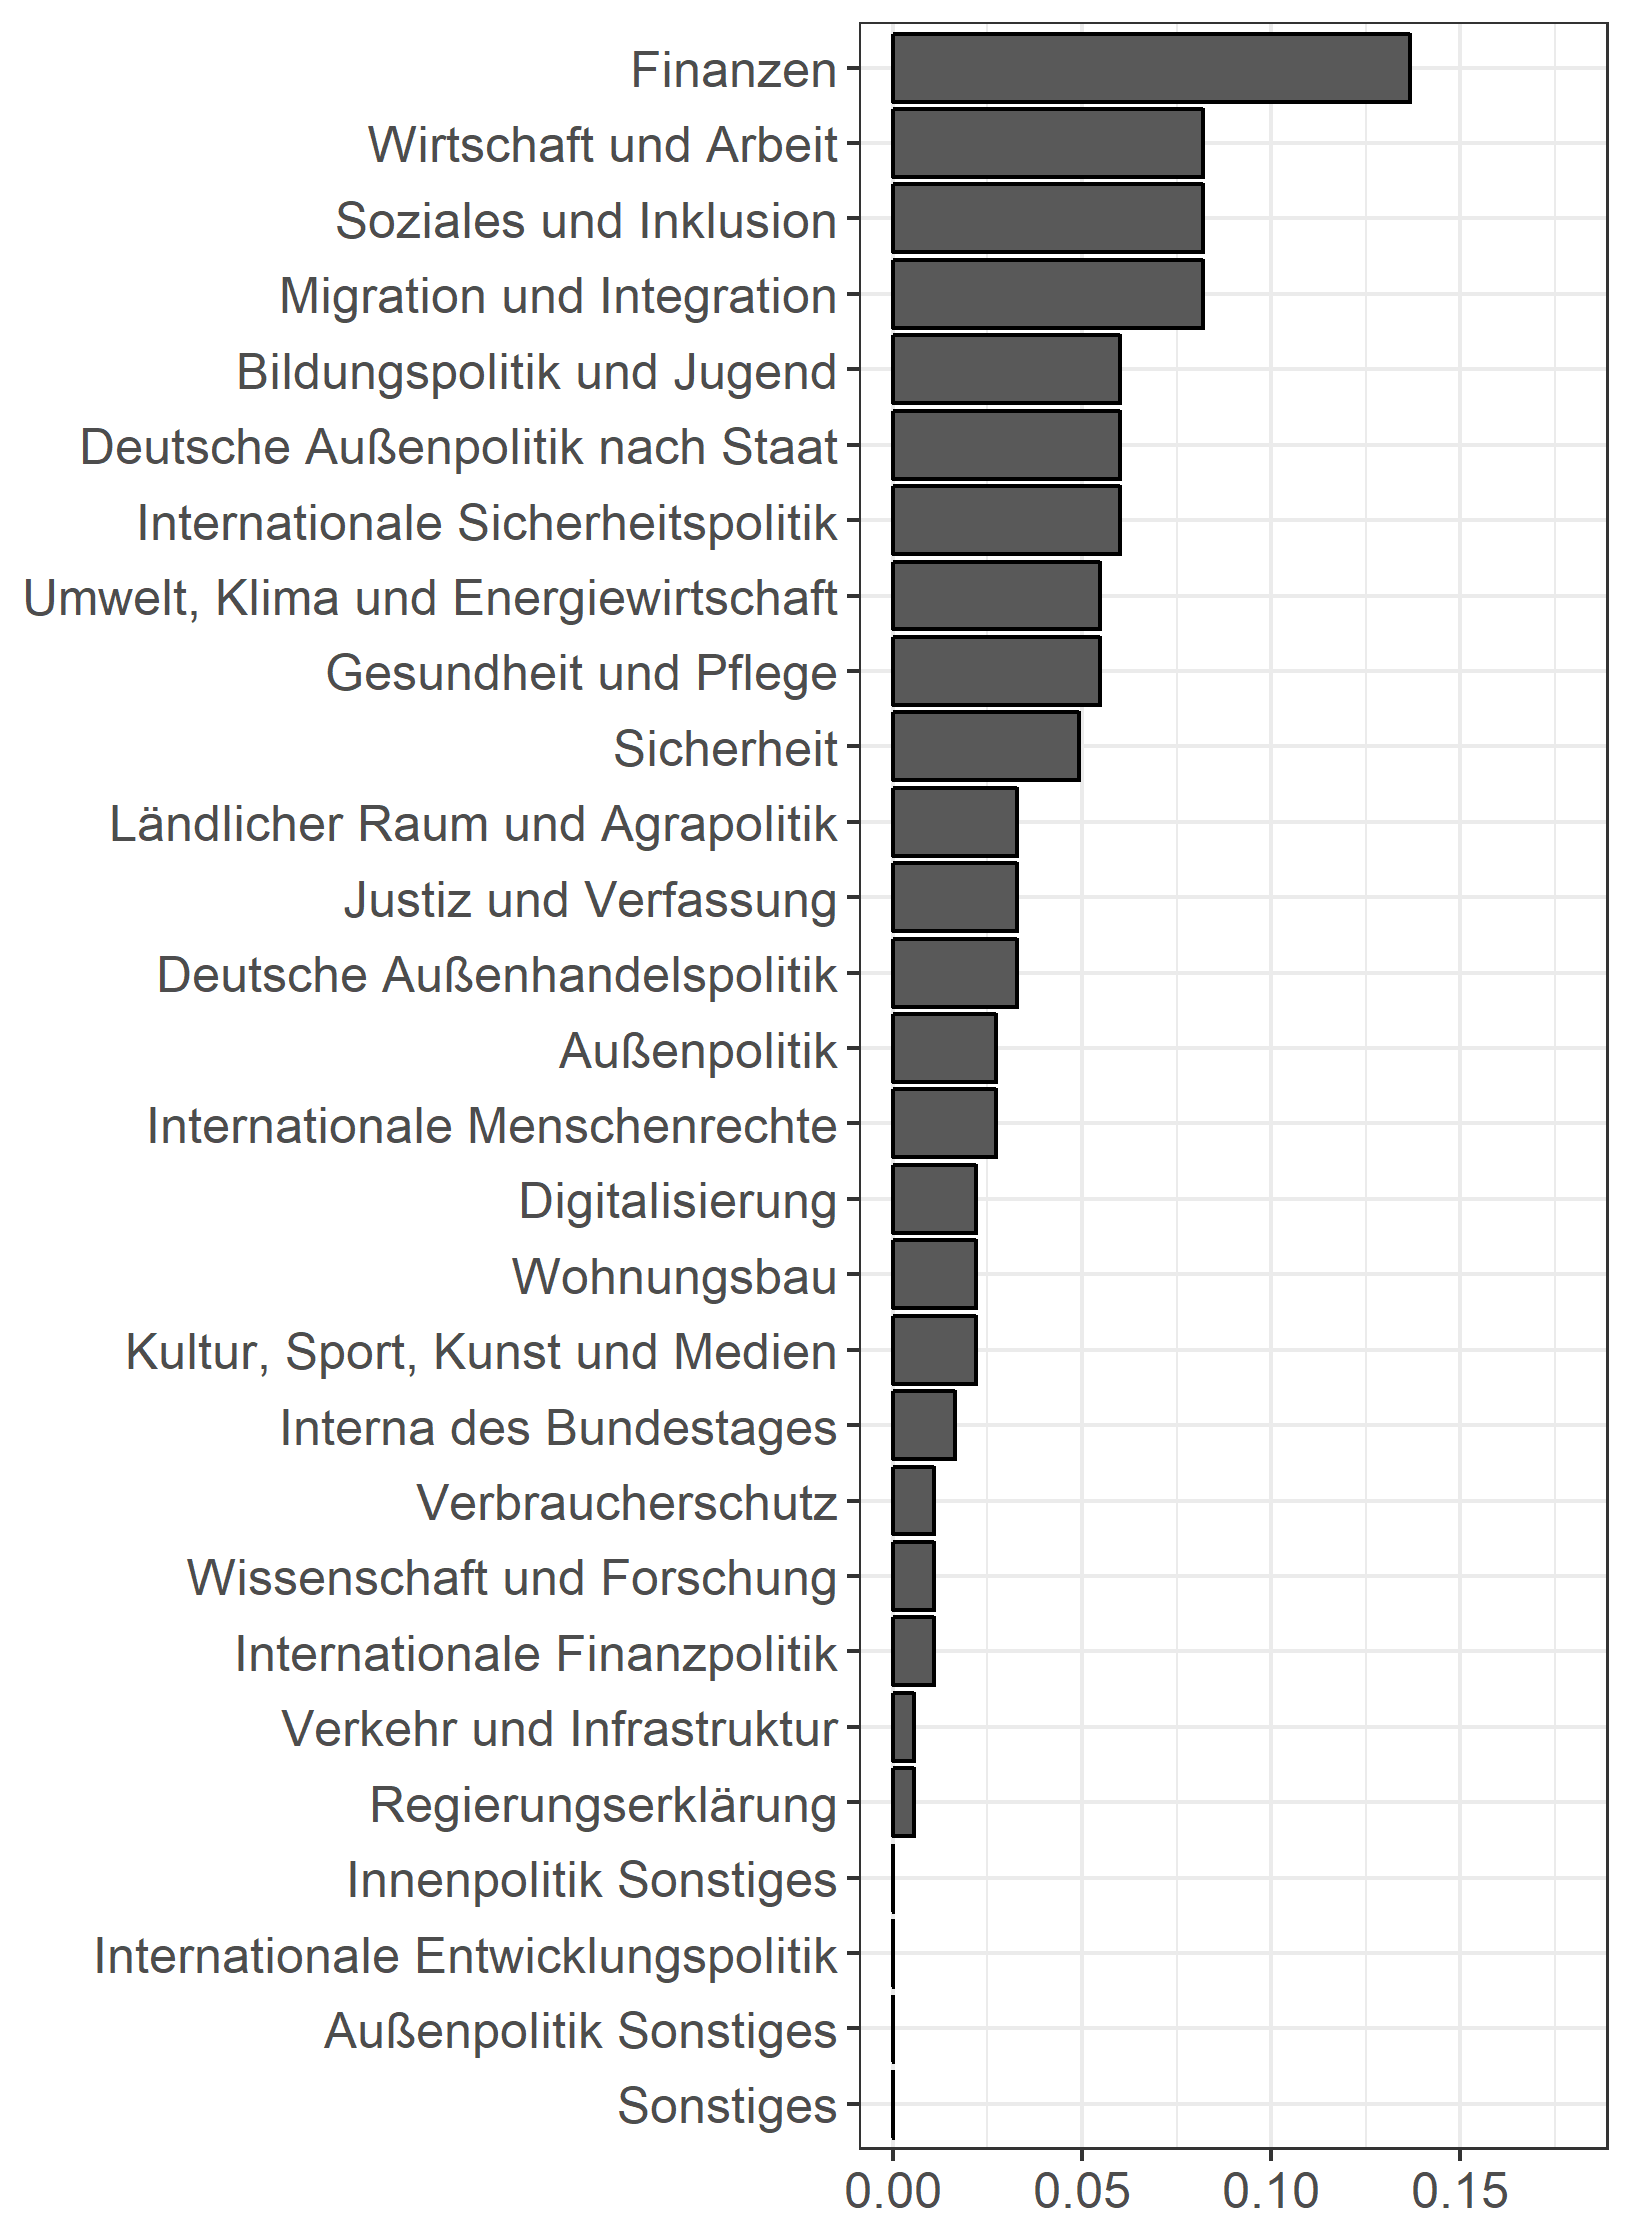
\includegraphics[width=0.29\textwidth]{Grafiken/Inhalt14.png}}
	\caption{Vergleich der Inhalte}
\end{figure}

Die Hypothese, dass seit dem Einzug der AfD über weniger Themen im Bundestag debattiert wird, lässt sich aus den Grafiken nicht erschließen. Dass bestimmte Themen den gesamten Ablauf im Bundestag dominieren und damit die Behandlung von diversen Problemen behindern, ließe sich bestätigen, wenn sich in der Grafik von 2017 einzelne Themen von den anderen abheben würden. Hier jedoch ist das genaue Gegenteil zu beobachten; 2017 scheinen die Themen sogar noch gleicher verteilter zu sein und damit wird breiter über mehrere Themen diskutiert. Allerdings kann hierbei keine Aussage darüber getroffen werden, ob die Themen, die in den Bundestagsreden behandelt werden auch vom Ablauf vorgesehen sind. Es könnte zu einer Behinderung von konstruktiven Debatten kommen, wenn Parteien entweder am Tagesordnungspunkt vorbei reden, oder aber Themen, die nicht im notwendigen Zusammenhang mit der anstehenden Debatte stehen mit in diese einbeziehen und so den Diskurs lähmen.  


\subsubsection{Hypothese 1b: Inhaltliche Distanz zum Tagesordnungspunkt}

Die Distanz zum Tagesordnungspunkt ist für uns definiert durch die Häufigkeit von Redeinhalten, die vom Inhalt des Tagesordnungspunktes abweichen, geteilt durch die Anzahl aller Themen. War in einer Debatte vom Tagesordnungspunkt beispielsweise Justiz vorhergesehen und eine Partei redet über Justiz und Verfassung, aber auch über Wirtschaft und Arbeit, dann ist die Distanz zum Tagesordnungspunkt 0.75 \\

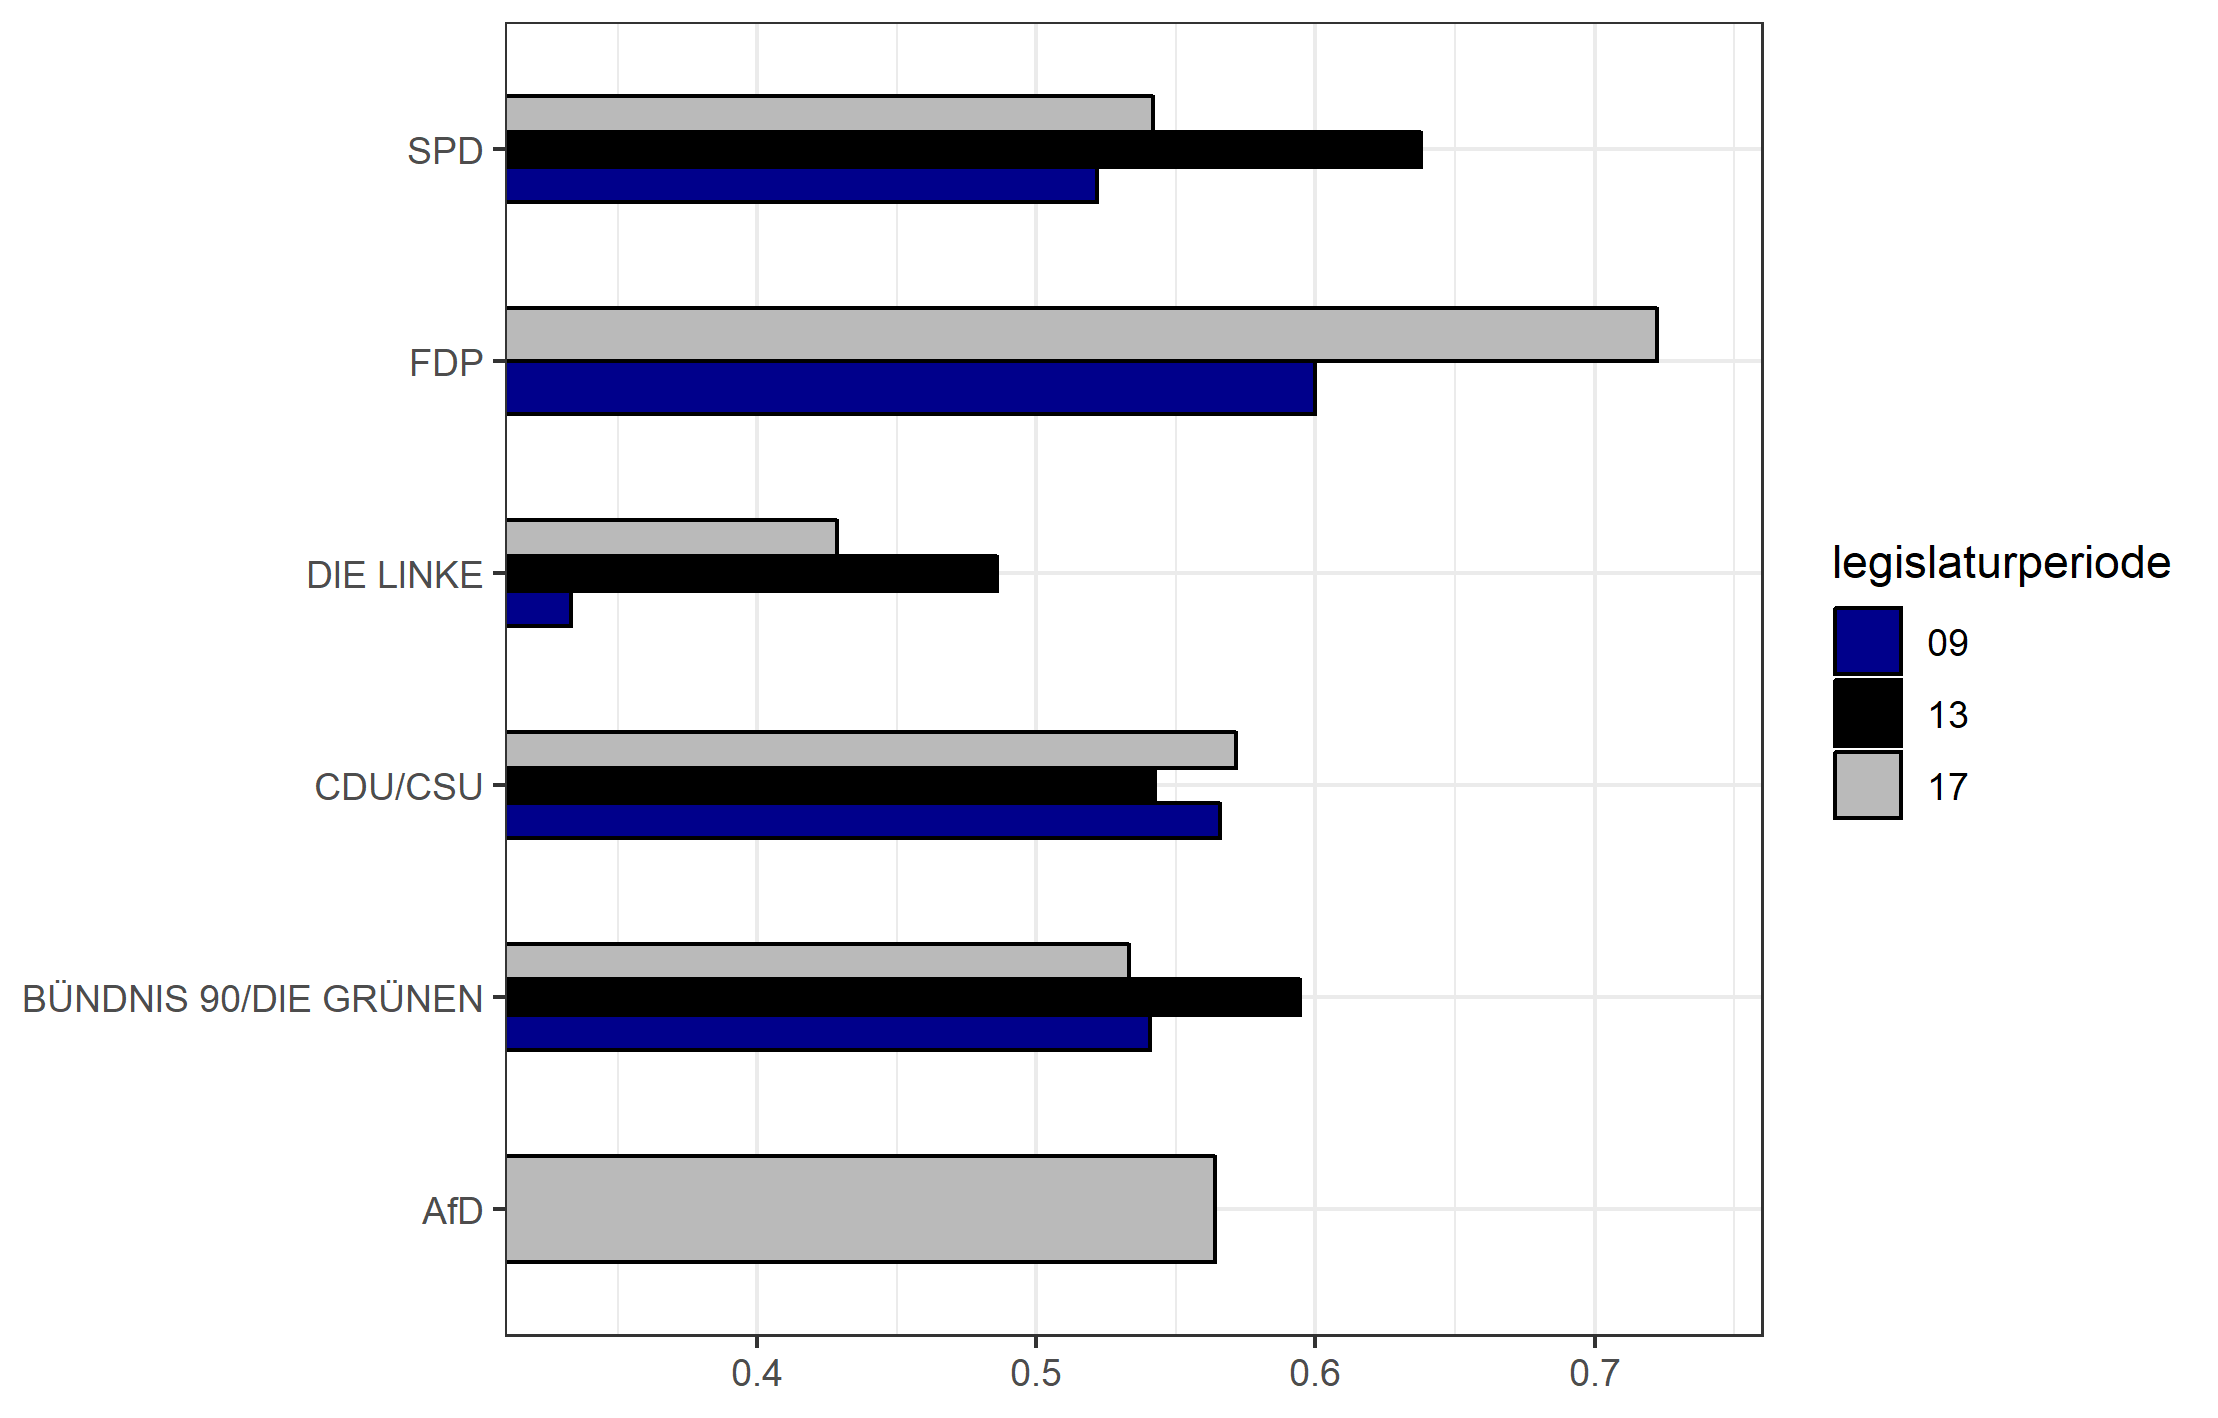
\includegraphics[width=\linewidth]{Grafiken/distop.png}\\

Es zeigt sich, dass die FDP am häufigsten am Tagesordnungspunkt vorbei diskutiert. 



\subsubsection{Hypothese 1c: Lenkung von Themen}
{\bfseries Methodologie Hypothese 1c:} Zur Überprüfung der Hypothese ist eine Netzwerkgraphik geeignet, da sie Aufschlüsse darüber gibt, welche Themen von Parteien gemeinsam mit anderen Themen verwendet werden. Man würde erwarten, dass das Thema Finanzen im Netzwerk in der Mitte steht und mit vielen Themen verbunden ist, da es in den Bundestagsdebatten egal bei welchen Thema häufig um die Frage der Finanzierung geht. Alle Abweichungen davon, zeigen eine Tendenz der Partei andere Themen häufiger in Debatten zu mogeln. Zur Messung welche Themen von welcher Partei gemeinsam verwendet werden braucht es eine größere Menge von kodierten Reden, als in der Stichprobe erreicht wurde. Daher wurde für diese Hypothese ein diktionär-basierter Ansatz verwendet, um zu ermitteln welche Themen in der Debatte behandelt wurden. Die Annahme besteht darin, dass häufiger Wörter aus der richtigen themenspezifischen Wortgruppen vorkommen, als aus anderen, selbst wenn es eine Schnittmenge zwischen den Wortgruppen gibt. Dafür wurden mit dem Latent-Semantic-Scaling Ansatz von \cite{watanabeSemisupevisedModelDocument2018} themenspezifische Wörterbücher erstellt, die jeweils 500 Wörter enthalten. Aus den Wörtern: "umwelt*","energie*","klima*","nachhaltig*","kohle*","emission*","abgase*" beispielsweise sind folgende Wörter entstanden, die zufällig aus den 500 ausgewählt wurden: \\

\begin{center}
\fbox{\parbox{\linewidth} {\noindent
		"braunkohle"               "umweltverträglich"        "subventionen"             "umweltminister"          
		"klimaschutzziel"                       "nachhaltigkeitsziele"    
		"energiepolitisches"       "umweltfragen"             "umweltfreundlich"         "energiesystem"                         "stroms"                   "grundlast"                "gesundheit"              
		"emissions"                "klimaflüchtlinge"         "ökologisch"               "klimaschutzfinanzierung" 
		"umweltbedingungen"        "natur"                    "ausbau"                   "eeg-umlage"              
		"regenerativer"            "lebensgrundlagen"                  "strommarkt"              
		"ambitionierten"           "nachhaltigkeitsstrategie"
}}\\
\end{center}

Aus diesen Wörtern wurde für jede Rede festgelegt zu welchen Prozentanteil die Rede aus Wörtern der jeweiligen themenspezifischen Wortgruppen besteht. Wenn eine Wortgruppe zu mindestens 20\% vorkommt, wurde das Thema als vorkommend gezählt. Anschließend wurde die Matrix transponiert und mit sich selbst multipliziert. Aus der resultierenden Co-Occurrence Matrix wurde der Netzwerkplot gebildet, wobei eine bestimmte Grenze an zusammen auftretenden Themen überschritten werden musste, dass eine Verbindung eingetragen wurde.   

\begin{center}
\begin{figure} [H]
	\subfigure[Gesamt]{\includegraphics[width=0.75\linewidth]{Grafiken/Themen_Gesamt.PNG}}
\end{figure}

\begin{figure} [H]
	\subfigure[AfD]{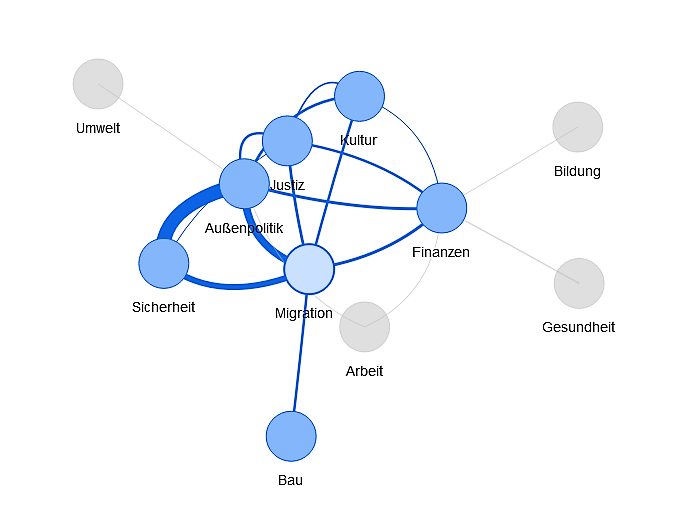
\includegraphics[width=0.75\linewidth]{Grafiken/Themen_AfD.PNG}}
\end{figure}
\end{center}


Die erste Grafik entspricht der Erwartung, dass alle Themen in einer Verbindung mit dem Thema Finanzen stehen, da es oft um die Frage der Finanzierung von Maßnahmen geht. Die zweite Grafik zeigt, wie die AfD von diesem "Normalzustand" abweicht und das Thema Migration in vielen anderen Themenbereichen vorkommt. Finanzen sind immer noch wichtig, aber haben keine zentrale Position mehr in dem Netzwerk. Das Bermudadreieck aus Sicherheit, Außenpolitik und Migration scheint die anderen Themen zu verschlingen. Die AfD schafft es Verbindungen zwischen Themen herzustellen, die im ersten Moment nicht notwendigerweise zusammengehörig erscheinen. Zum Beispiel erscheint die Verbindung zwischen Bau und Migration im ersten Moment fragwürdig. Dafür an dieser Stelle drei qualitative Beispiele aus der Co-Occurrence Matrix, in denen die AfD vom Thema Bau, Kultur und Justiz auf das Thema Migration lenkt.  

\noindent Beispiel für eine Rede, die das Thema Wohnen (Bau) auf das Thema Migration lenkt. Redner ist Marc Bernhard (AfD):\\

\fbox{\parbox{\linewidth} {\noindent Allein 1 Million Wohnungen davon werden für die rund 2 Millionen illegal eingereisten Migranten benötigt, die die Regierung in den letzten drei Jahren ins Land gelassen hat. (Michael Grosse-Brömer [CDU/CSU]: Der Migrationstextbaustein! – Ulli Nissen [SPD]: Was reden Sie da für einen Unfug! – Christian Kühn [Tübingen] [BÜNDNIS 90/DIE GRÜNEN]: Woher kommt die Zahl?)– Ja, regen Sie sich nur auf. – Die restlichen 500 000 Wohnungen reichen nicht einmal für den Familiennachzug, geschweige denn für die weitere illegale Zuwanderung, wenn diese nicht gestoppt wird.(Beifall bei der AfD) Die Bundesregierung spielt also die deutsche Bevölkerung und die Flüchtlinge auf dem Wohnungsmarkt gegeneinander aus.}}\\


\noindent Beispiel für eine Rede, die das Thema Kultur auf das Thema Migration lenkt:\\

\fbox{\parbox{\linewidth} {\noindent Beatrix von Storch (AfD): Sehr geehrter Herr Präsident! Sehr geehrte Damen und Herren! Jüdisches Leben gehört zu Deutschland. Die älteste jüdische Gemeinde siedelte in Mainz in der ersten Hälfte des 10. Jahrhunderts. Das jüdische Leben war schon Teil von Deutschland, als Deutschland sich als Nation gründete. – Der Islam war historisch nie zu Deutschland gehörend, das Judentum immer; das ist eine historische Tatsache.Nach dem Zivilisationsbruch des Nationalsozialismus wollen wir, dass jüdisches Leben in Deutschland wieder blüht. Gerade angesichts der Tatsache, dass es in Westeuropa durch die Islamisierung in seiner Existenz bedroht ist, müssen wir mit aller Kraft gegensteuern.}}\\

\noindent Beispiel für eine Rede, die das Thema Justiz auf das Thema Migration lenkt: \\

\fbox{\parbox{\linewidth} {\noindent Matthias Peterka (AfD):Sehr geehrter Herr Präsident! Werte verbliebene Kollegen! Der vorliegende Gesetzentwurf soll angeblich dafür sorgen, dass deutsche Verwaltungsgerichte nicht mehr heillos überlastet werden. Er stammt gleichzeitig von der Partei, die diesen Missstand am fröhlichsten, am buntesten und – um es auf den Punkt zu bringen – am ideologischsten herbeigeführt hat.(Beifall bei der AfD – Katja Keul [BÜNDNIS 90/DIE GRÜNEN]: Ach, wegen der Grünen sind die alle gekommen! – Ulli Nissen [SPD]: Vielleicht fällt Ihnen mal etwas Neues ein!)Hier wird nicht nur der Bock zum Gärtner gemacht, hier macht sich der Bock gleich selbst dazu.(Tabea Rößner [BÜNDNIS 90/DIE GRÜNEN]: So ein Quatsch!)Ich persönlich würde gerne glauben, dass Sie die Ausführungen in der Begründung auch ernst meinen, dass Ihnen ein Licht in dieser Sache aufgegangen ist. Aber es tut mir leid, ich bin nicht ganz naiv.Sie beklagen, dass die Explosion bei der Zahl der eingehenden Asylklagen drei Viertel der laufenden Kapazität der Verwaltungsgerichte lahmlegt. Doch dies wird sodann als gerichtsorganisatorische Herausforderung verniedlicht. Ich nenne es Rechtsstaatsversagen auf ganzer Linie und mit Ansage.(Beifall bei der AfD)Dem Normalbürger außerhalb der heiligen Kuh Asylrecht wird der Abbau des Rechtsschutzes seit Jahren in homöopathischen Dosen verabreicht und von dem auch so geschluckt. Das ist der bloße Verdrängungseffekt.}}\\


\subsection {Hypothese 2: Sprachverständlichkeit}

{\bfseries Methodologie Hypothese 2:} Zur Überprüfung der Sprachverständlichkeit wurden alle Reden der momentanen Legislaturperiode nach Monaten und Parteien gruppiert und anschließend, in Silben, Wörter und Sätze aufgegliedert. Aus diesen Daten wurde der deutsche FLESCH-Index berechnet, eine von \cite{amstadWieVerstandlichSind1978} an die deutsche Sprache angepasste Variation vom FLESCH-Index, der als einer der etabliertesten Readability-Indizes in der Sprachverständlichkeitsforschung gilt. Die
Werte wurden mit der Funktion \texttt{flesch()} mit dem Parameter {\verb de } aus dem R-Package KoRpus (\cite{michalkeKoRpusPackageText2018}) berechnet.\\

\fbox{\parbox{\linewidth}{\[r_{German} = 80 - 58.5 * \frac{y}{w} - \frac{w}{s} \] \textbf{w}: Gesamtanzahl von Wörtern \textbf{y}: Gesamtanzahl von Silben \textbf{s}: Gesamtanzahl von Sätzen}}\\


\noindent Dafür wurden die Texte zunächst mit der \texttt{tokenize()} funktion aus dem ``koRpus'' Package in Buchstaben aufgeteilt. 

Der FLESCH-Index ist aus deshalb gut anwendbar, weil er leicht zu interpretieren ist. Jeder Wert kann in etwa einem Alter zugeordnet werden, das erforderlich ist, um die Texte zu verstehen. 

\begin{longtable}[]{@{}lll@{}}
	\toprule
	Flesch-Reading-Ease-Score Von \ldots{} bis unter \ldots{} & Lesbarkeit &
	Verständlich für\tabularnewline
	\midrule
	\endhead
	0--30 & Sehr schwer & Akademiker\tabularnewline
	30--50 & Schwer &\tabularnewline
	50--60 & Mittelschwer &\tabularnewline
	60--70 & Mittel & 13--15-jährige Schüler\tabularnewline
	70--80 & Mittelleicht &\tabularnewline
	80--90 & Leicht &\tabularnewline
	90--100 & Sehr leicht & 11-jährige Schüler\tabularnewline
	\bottomrule
\end{longtable}


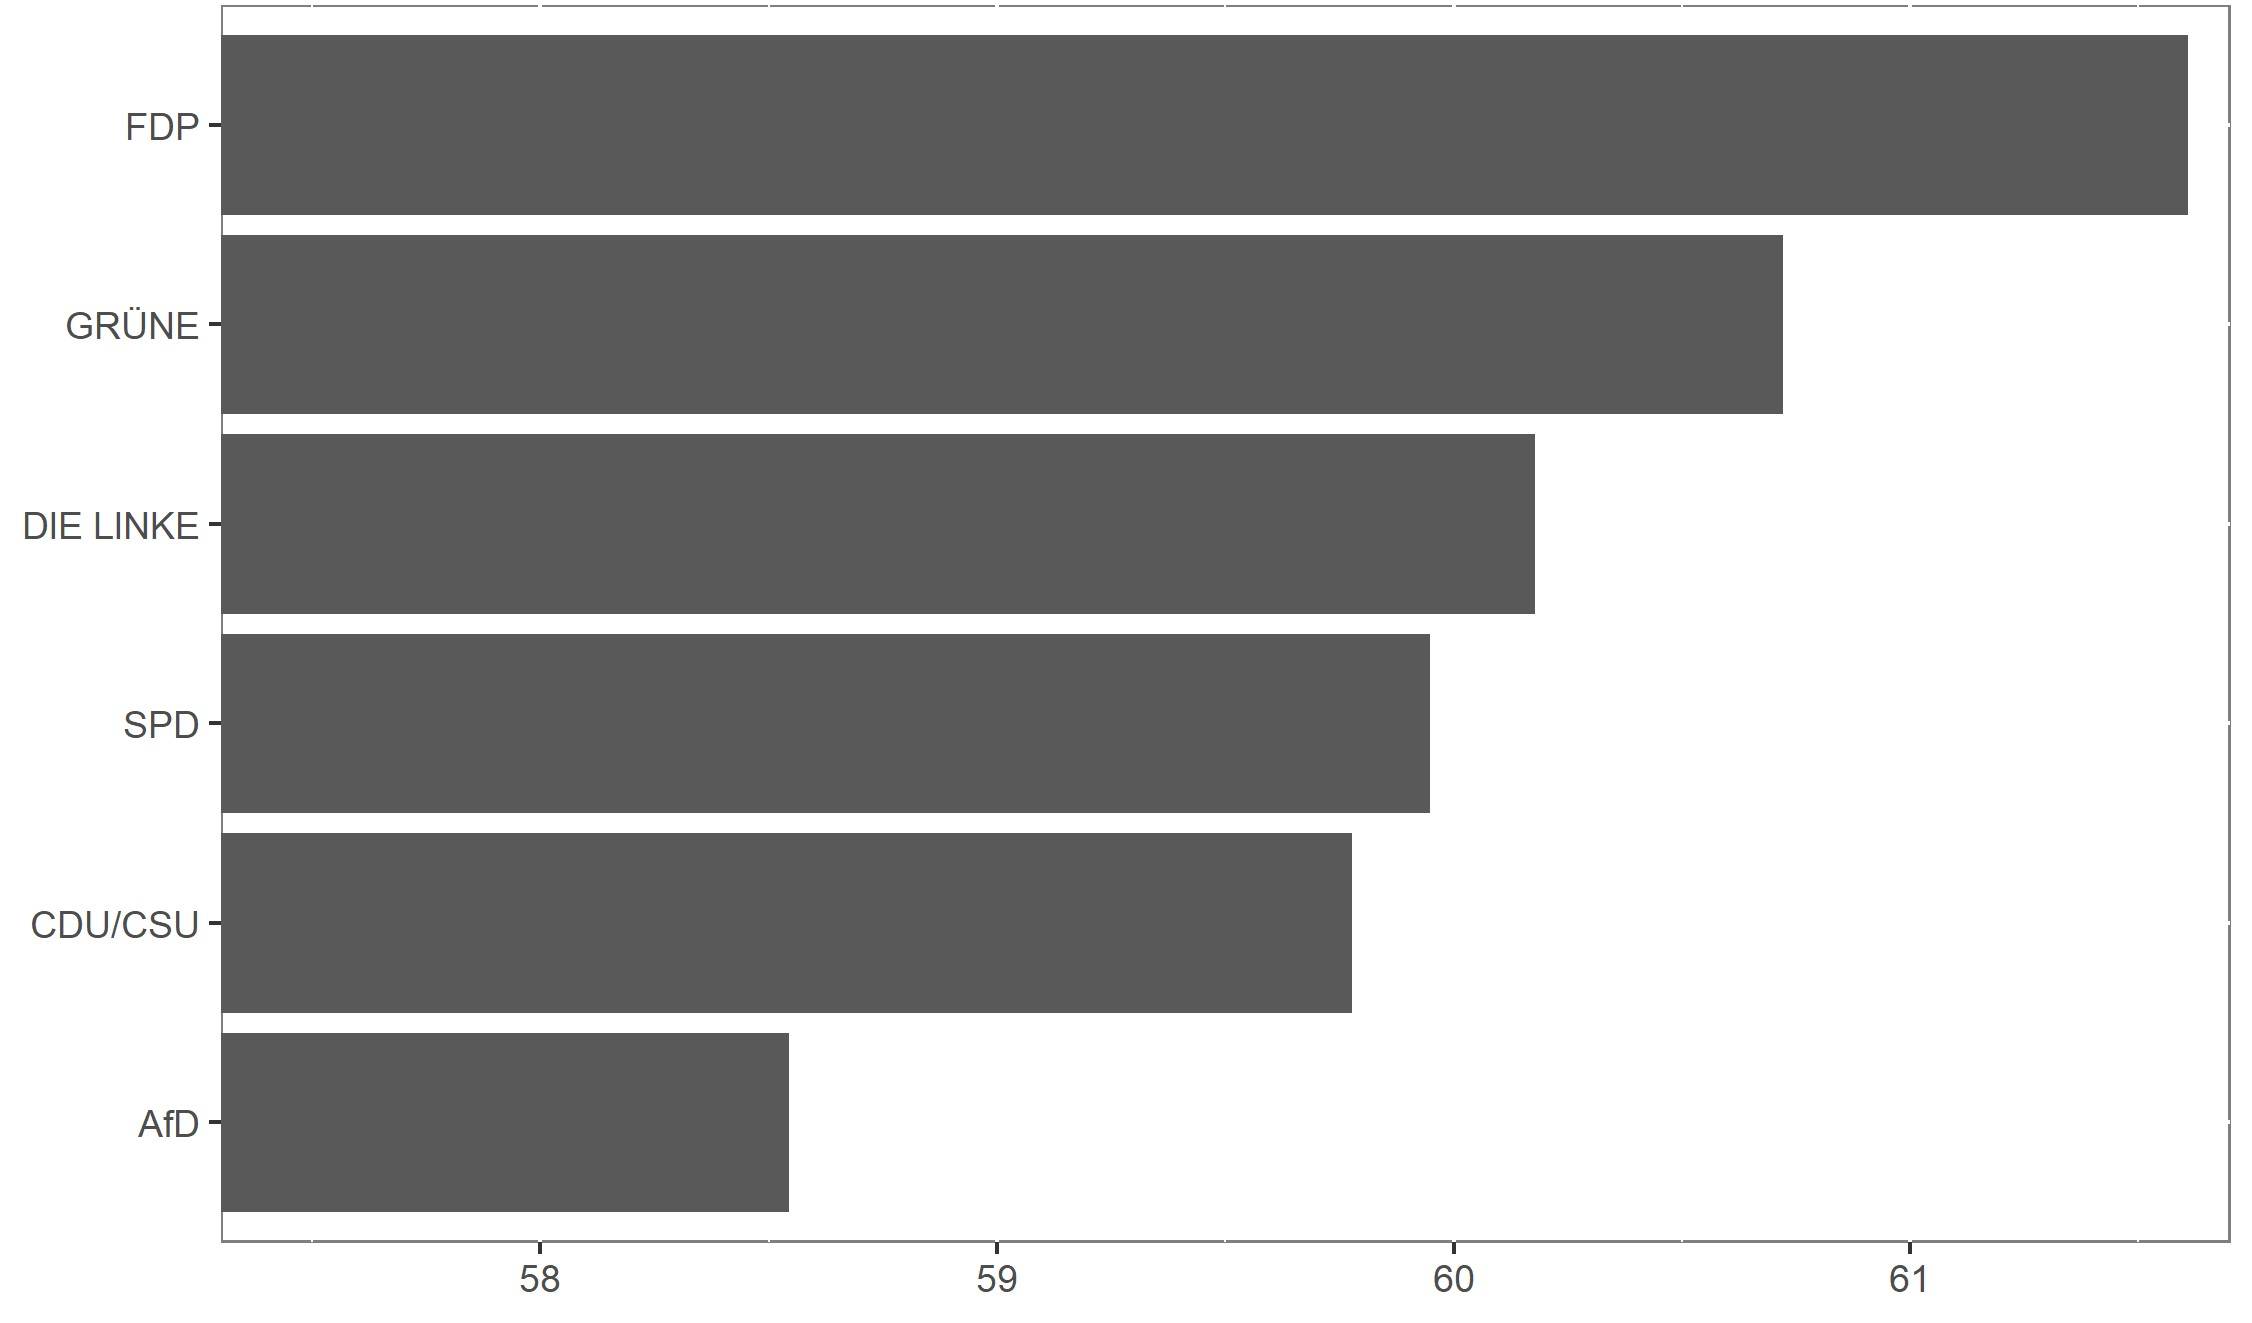
\includegraphics[width=\linewidth]{Grafiken/Readability_line.jpg}\\

Die AfD hat den niedrigsten Flesch-Reading Wert und ist damit am einfachsten zu verstehen. Erwartet hat dies nur ein Teil unserer Gruppe. Es spricht einiges dafür, dass man bei der AfD mit der hohen Anzahl an Professoren ein hohen Wert erwarten könnte. Auf der anderen Seite ist die AfD eine populistische Partei, die durch eine einfache Sprache erfolgreich und verständlich bei der großen Masse sein möchte. Eine einfache Sprache ist dafür eine wichtige Voraussetzung. Die Validität der Ergebnisse ist dennoch zu hinterfragen, da der FLESCH-Index sehr einfach aufgebaut ist und weder Satzstrukturen, noch Fachwörter oder grammatikalische Eigenschaften berücksichtigt. 


\subsection{Hypothese 3: Isolation der Parteien}

{\bfseries Methodologie Hypothese 3:} Zur Überprüfung der Hypothese, welche Partei wie isoliert ist, wurden alle \verb 445.301  Interaktionen im Bundestag im Zeitraum von 2009-2017 analysiert. Zusätzlich wurden die häufigsten verwendeten Wörter der Parteien analysiert. \\

Folgende Interaktionen sind den Bundestagsprotokollen entnommen worden: 
\begin{center}
% latex table generated in R 3.5.0 by xtable 1.8-3 package
% Sun Nov 18 13:22:12 2018
\begin{table}[ht]
	\centering
	\begin{tabular}{lrrrrrrrl}
		\hline
		Partei & Beifall & Heiterkeit & Kommentar & Lachen & Widerspruch & Zuruf & Summe & Periode \\ 
		\hline
		\hline
		SPD & 12311 & 318 & 3346 & 231 & 109 & 373 & 16315 & 17-18 \\ 
		CDU/CSU & 11659 & 333 & 3847 & 112 &  53 & 223 & 16004 & 17-18 \\ 
		DIE LINKE & 9462 & 125 & 2927 & 142 & 107 & 367 & 12763 & 17-18 \\ 
		GRÜNE & 7417 & 131 & 4205 &  95 &  69 & 335 & 11917 & 17-18 \\ 
		FDP & 8470 & 258 & 2782 &  86 &  36 & 249 & 11632 & 17-18 \\ 
		AfD & 7074 & 129 & 3557 & 291 & 114 & 734 & 11165 & 17-18 \\ 
		\hline
		CDU/CSU & 32638 & 856 & 10018 & 234 & 150 & 1047 & 43812 & 13-17 \\ 
		SPD & 32217 & 934 & 6087 & 124 & 159 & 615 & 39407 & 13-17 \\ 
		GRÜNE & 14148 & 158 & 15363 & 116 & 131 & 791 & 29800 & 13-17 \\ 
		DIE LINKE & 20789 & 282 & 8218 & 153 & 210 & 1221 & 29451 & 13-17 \\ 
		\hline
		SPD & 27330 & 731 & 24078 & 863 & 496 & 2264 & 53064 & 09-13 \\ 
		CDU/CSU & 34131 & 633 & 13515 & 326 & 272 & 1584 & 48719 & 09-13 \\ 
		FDP & 32808 & 577 & 10484 & 333 & 280 & 1499 & 44323 & 09-13 \\ 
		DIE LINKE & 19275 & 308 & 7583 & 299 & 268 & 1199 & 27503 & 09-13 \\ 
		GRÜNE & 11716 & 199 & 13391 & 213 & 178 & 634 & 25537 & 09-13 \\ 
		\hline
	\end{tabular}
\end{table}
\end{center}

\subsubsection{Klatschen für andere Fraktionen}

 Beifall ist eine sehr deutliche Form der Zustimmung, die einfach zu erkennen und leicht interpretierbar ist. Klatscht eine Partei für eine andere, so lässt sich daraus schließen, dass die Partei der Rede zustimmt. Aus den Bundestagsprotokollen geht dabei hervor, welche Partei wann klatscht und ob die ganze Partei in den Beifall einstimmt, oder nur einzelne Abgeordnete. Unsere Analyse hat aus den Protokolle der vergangenen zwei Perioden ausgewertet, welche Partei für welche klatscht und damit Zustimmung signalisiert.   \\


\includegraphics[width=\linewidth]{Grafiken/13_17WerfürWen_prozent_bunt.png}\\
Es zeigt sich, dass die Koalitionsparteien am über alle drei Legislaturperioden hinweg am meisten für einander applaudieren. Allerdings wird der Beifall von SPD und CDU/CSU füreinander in der zweiten gemeinsamen Legislaturperiode kleiner.\\

\subsubsection{Klatschen für die eigene Fraktion}
 \noindent Je häufiger eine Partei für sich selbst klatscht im Verhältnis zum Klatschen für andere Parteien, desto eher ist sie in einer isolierten Position. Sie stimmt nur den eigenen Inhalten zu und hat kaum eine inhaltliche Position mit einer anderen Partei gemeinsam. Eine Analyse über den "Eigenklatschanteil" kann also Aufschluss darüber geben, wie isoliert eine Partei ist. \\

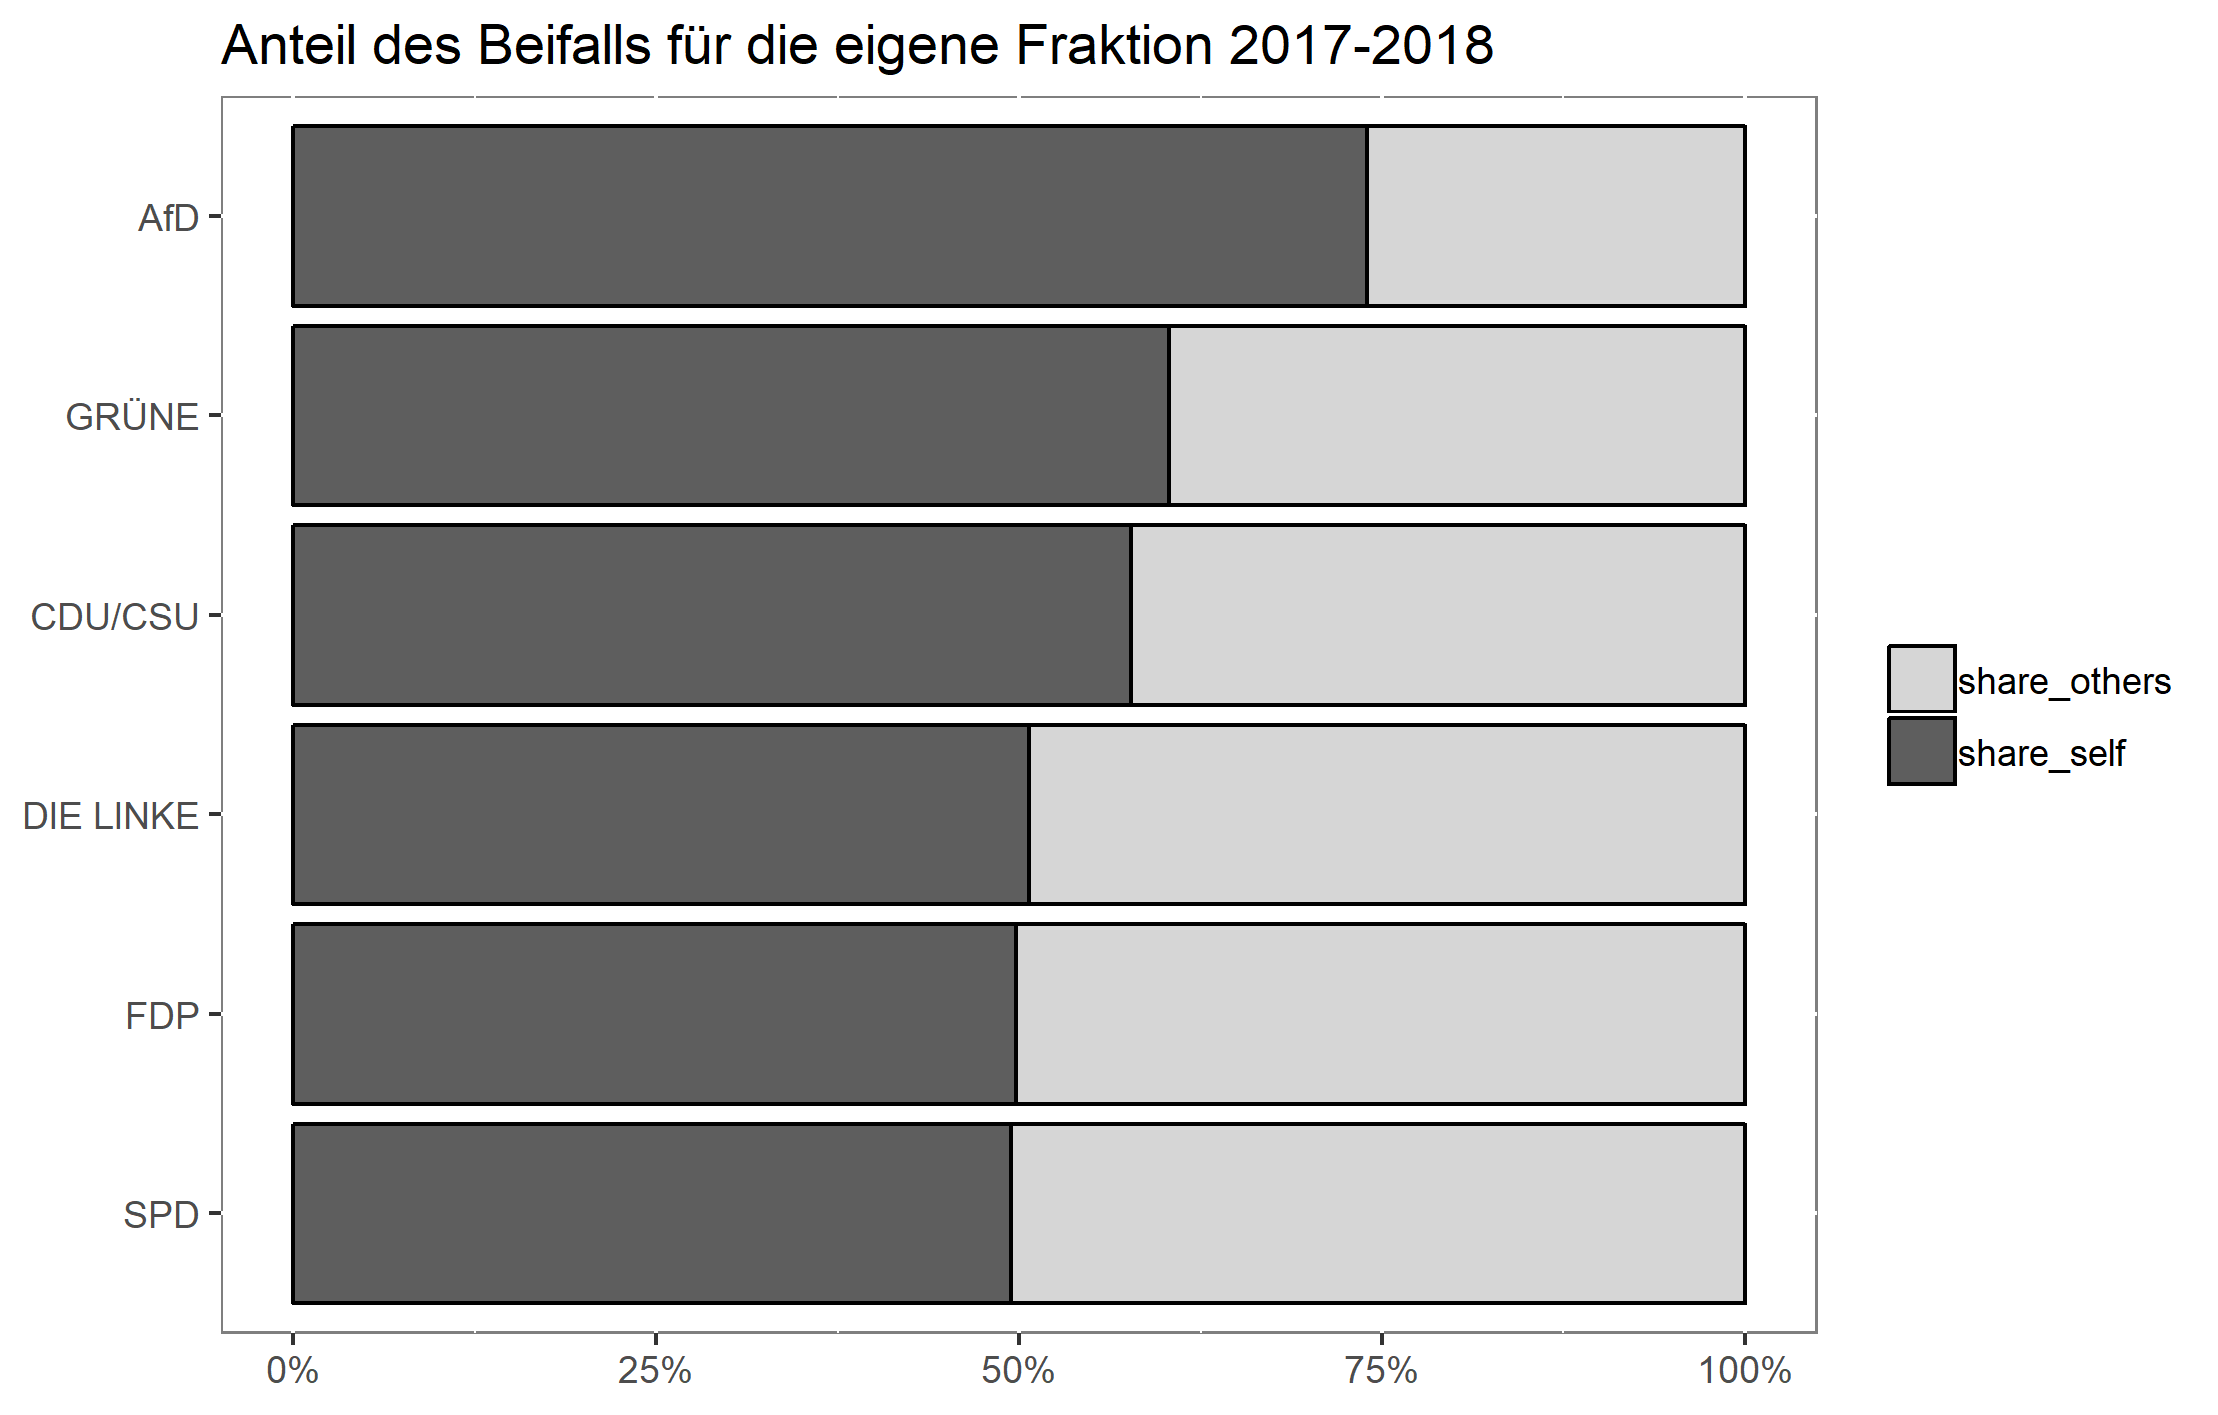
\includegraphics[width=\linewidth]{Grafiken/17_eigenklatschanteil.png}

Die AfD ist demnach die isolierteste Partei. Betrachtet man den "Eigenklatschanteil" im Zeitverlauf zeigt sich, dass auch andere Parteien sich in der momentanen Legislaturperiode zunehmend zu isolieren scheinen.\\
  
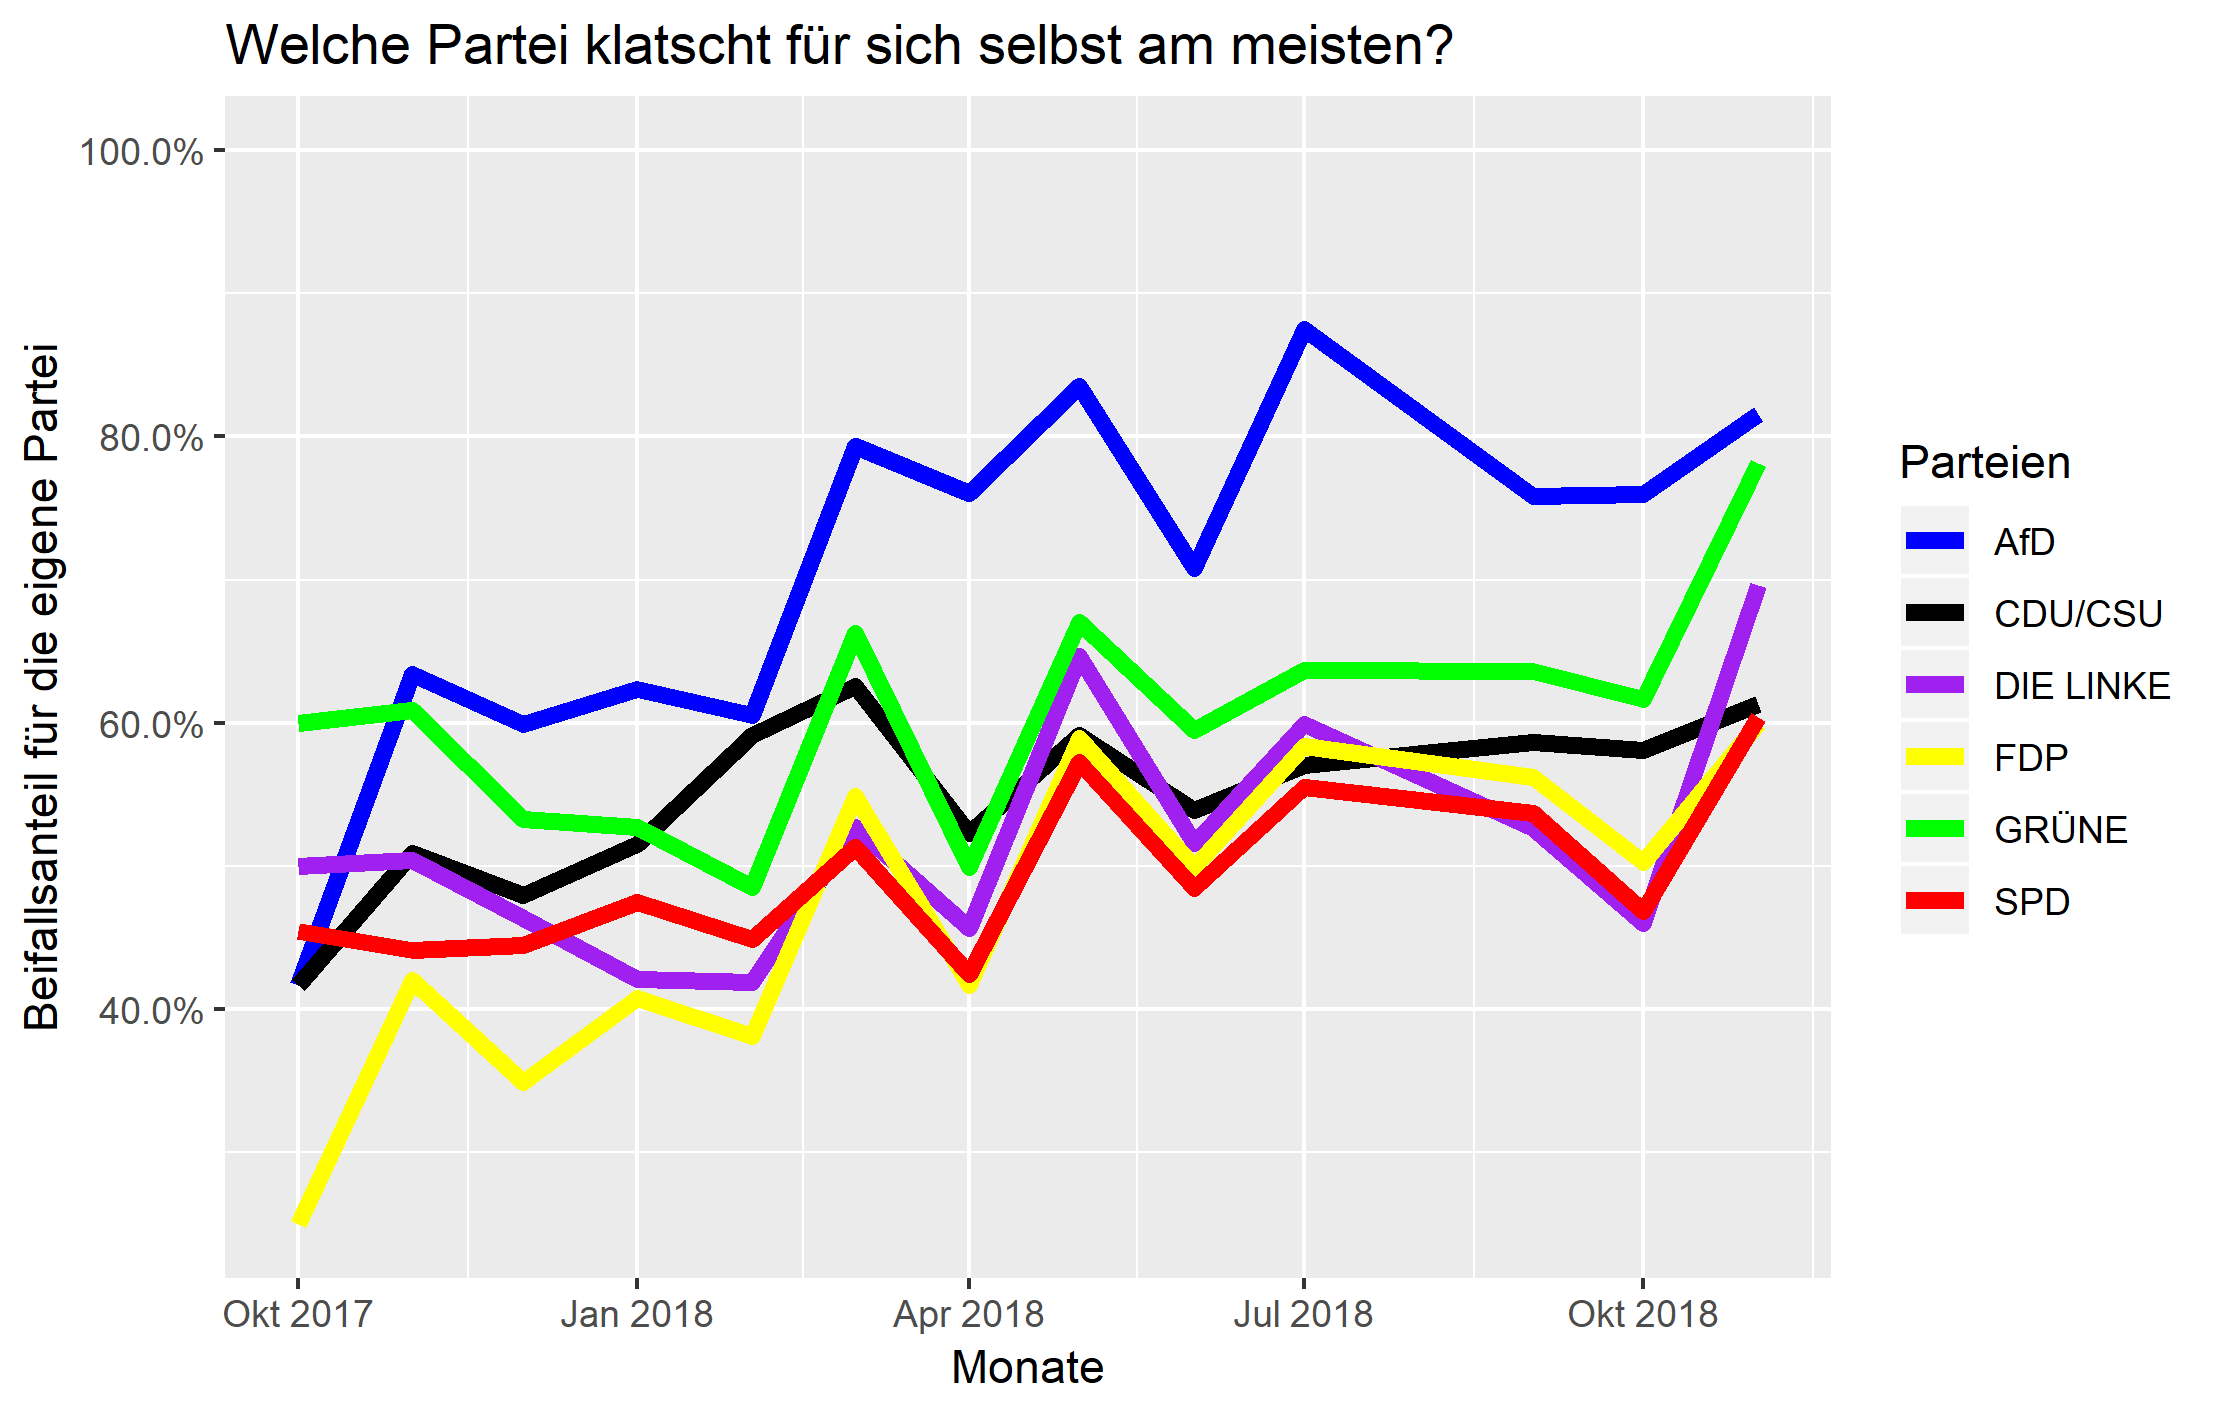
\includegraphics[width=\linewidth]{Grafiken/13_17Zeitverlauf_Klatschen.png}\\

\subsubsection{Geschlossenheit der Parteien}
Ein geschlossenes Auftreten von Parteien nur anhand von gemeinsamen Interaktionen fest zu machen, ist nur begrenzt aussagekräftig. Dennoch sind neben einem kohärenten Inhalt gemeinsame Aktionen ein deutliches Zeichen nach außen, ob eine Partei geschlossen auftritt, oder nicht. Gemeinsamer Beifall ist demnach ein Indikator für Geschlossenheit. \\

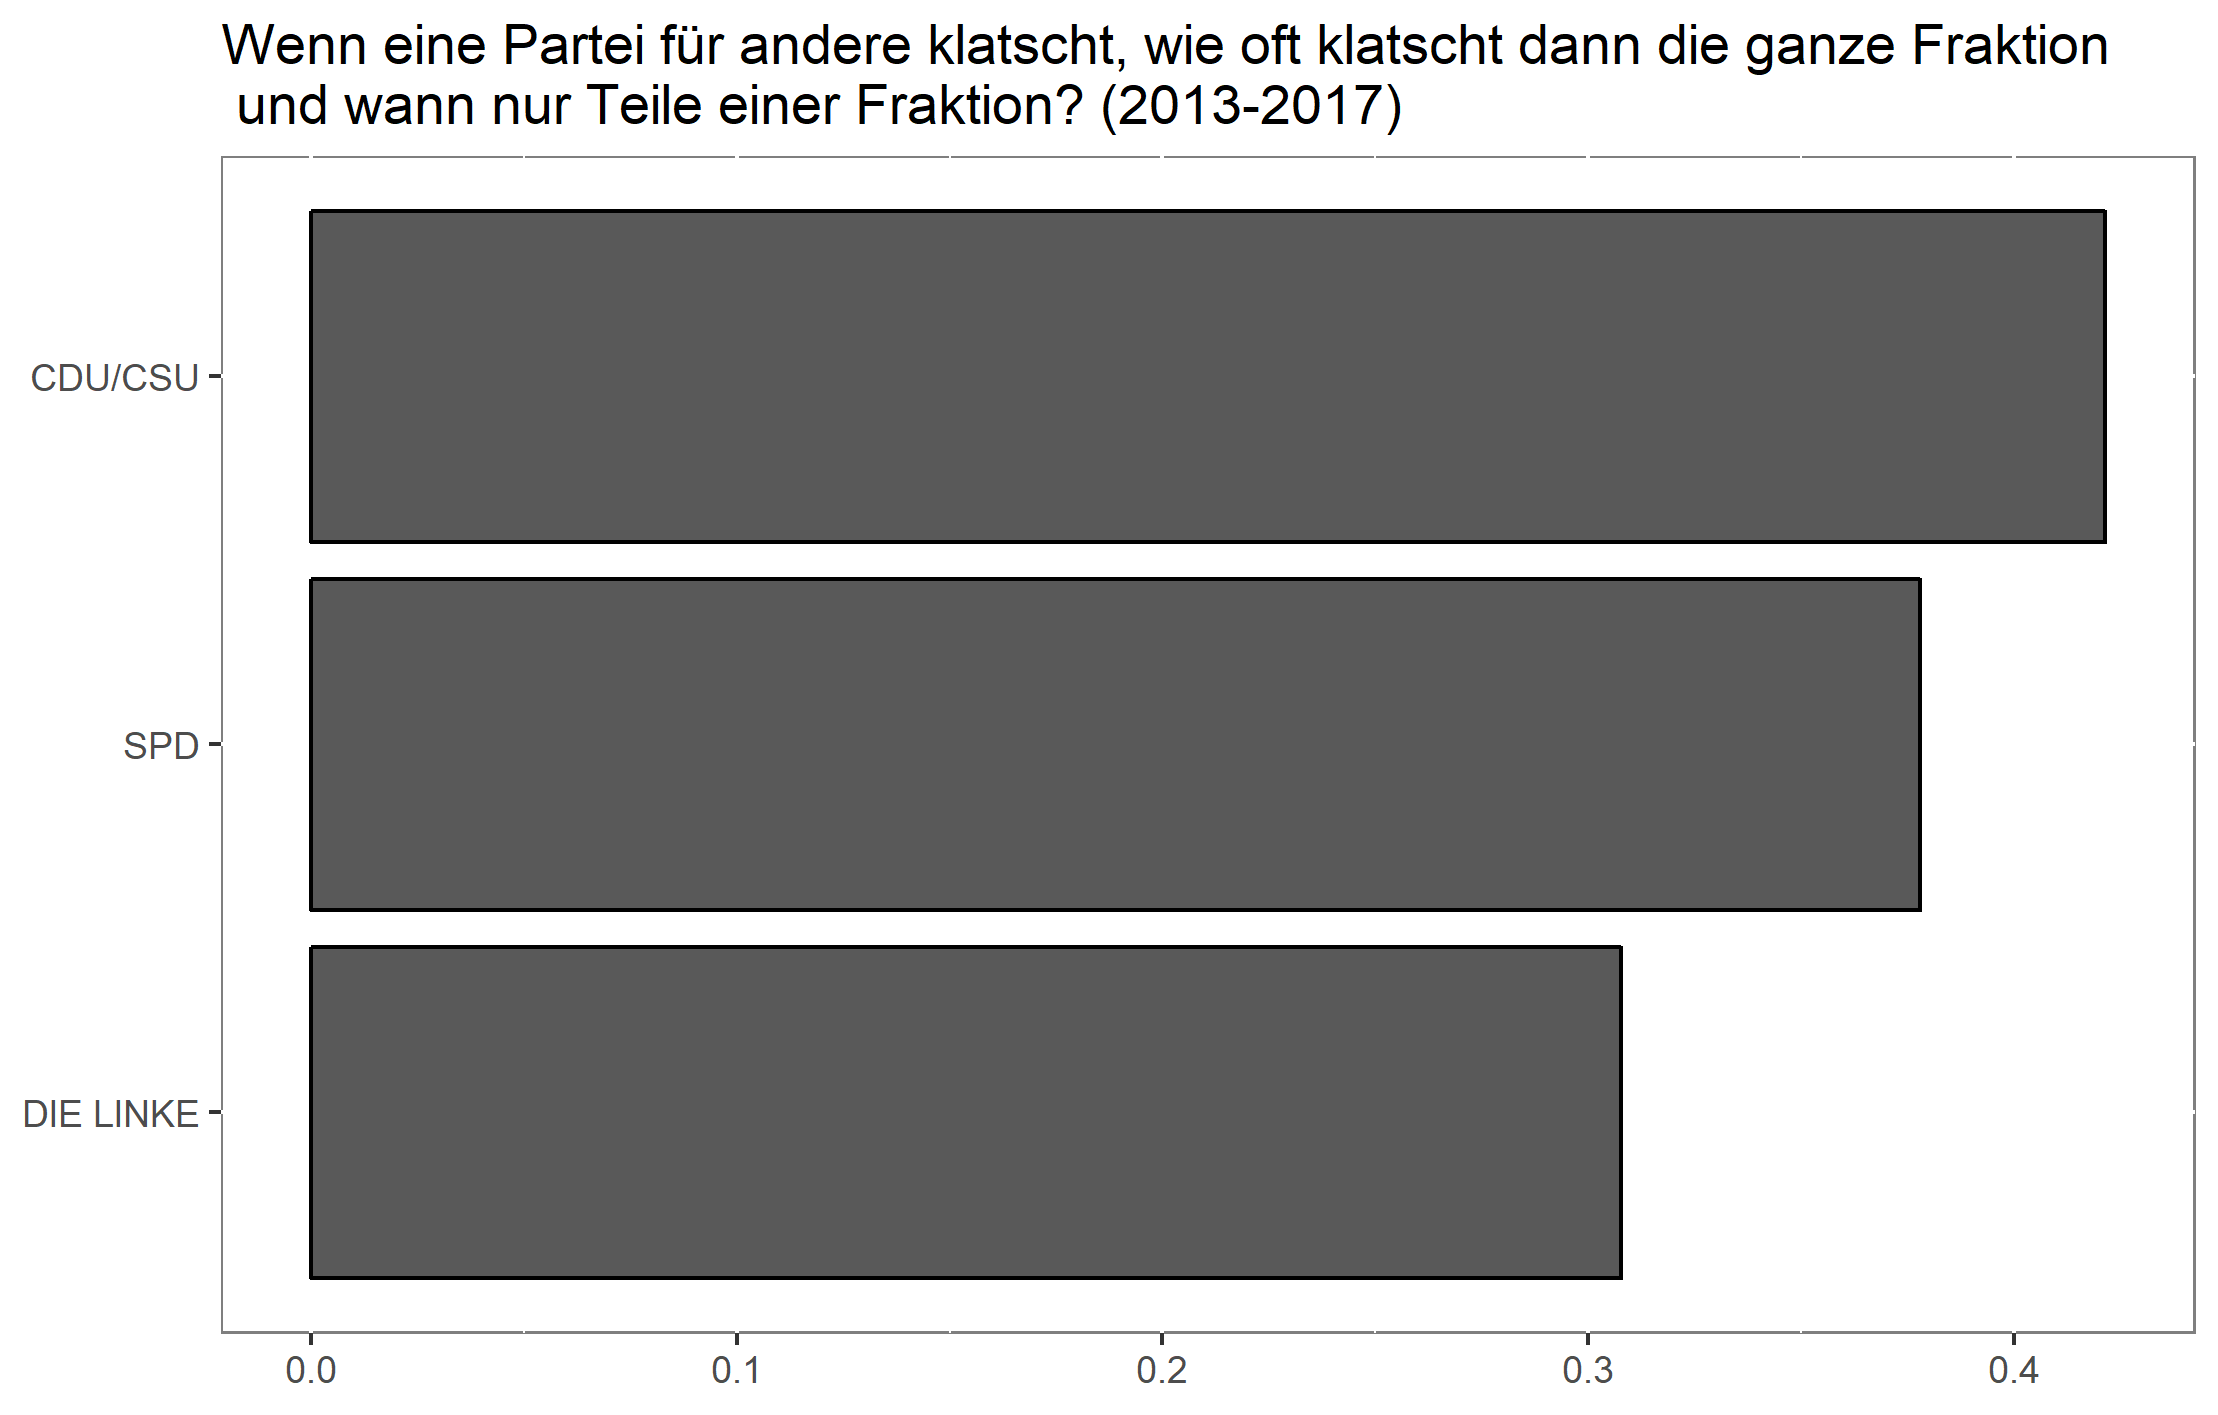
\includegraphics[width=0.5\linewidth]{Grafiken/Geschlossenheit13.png}
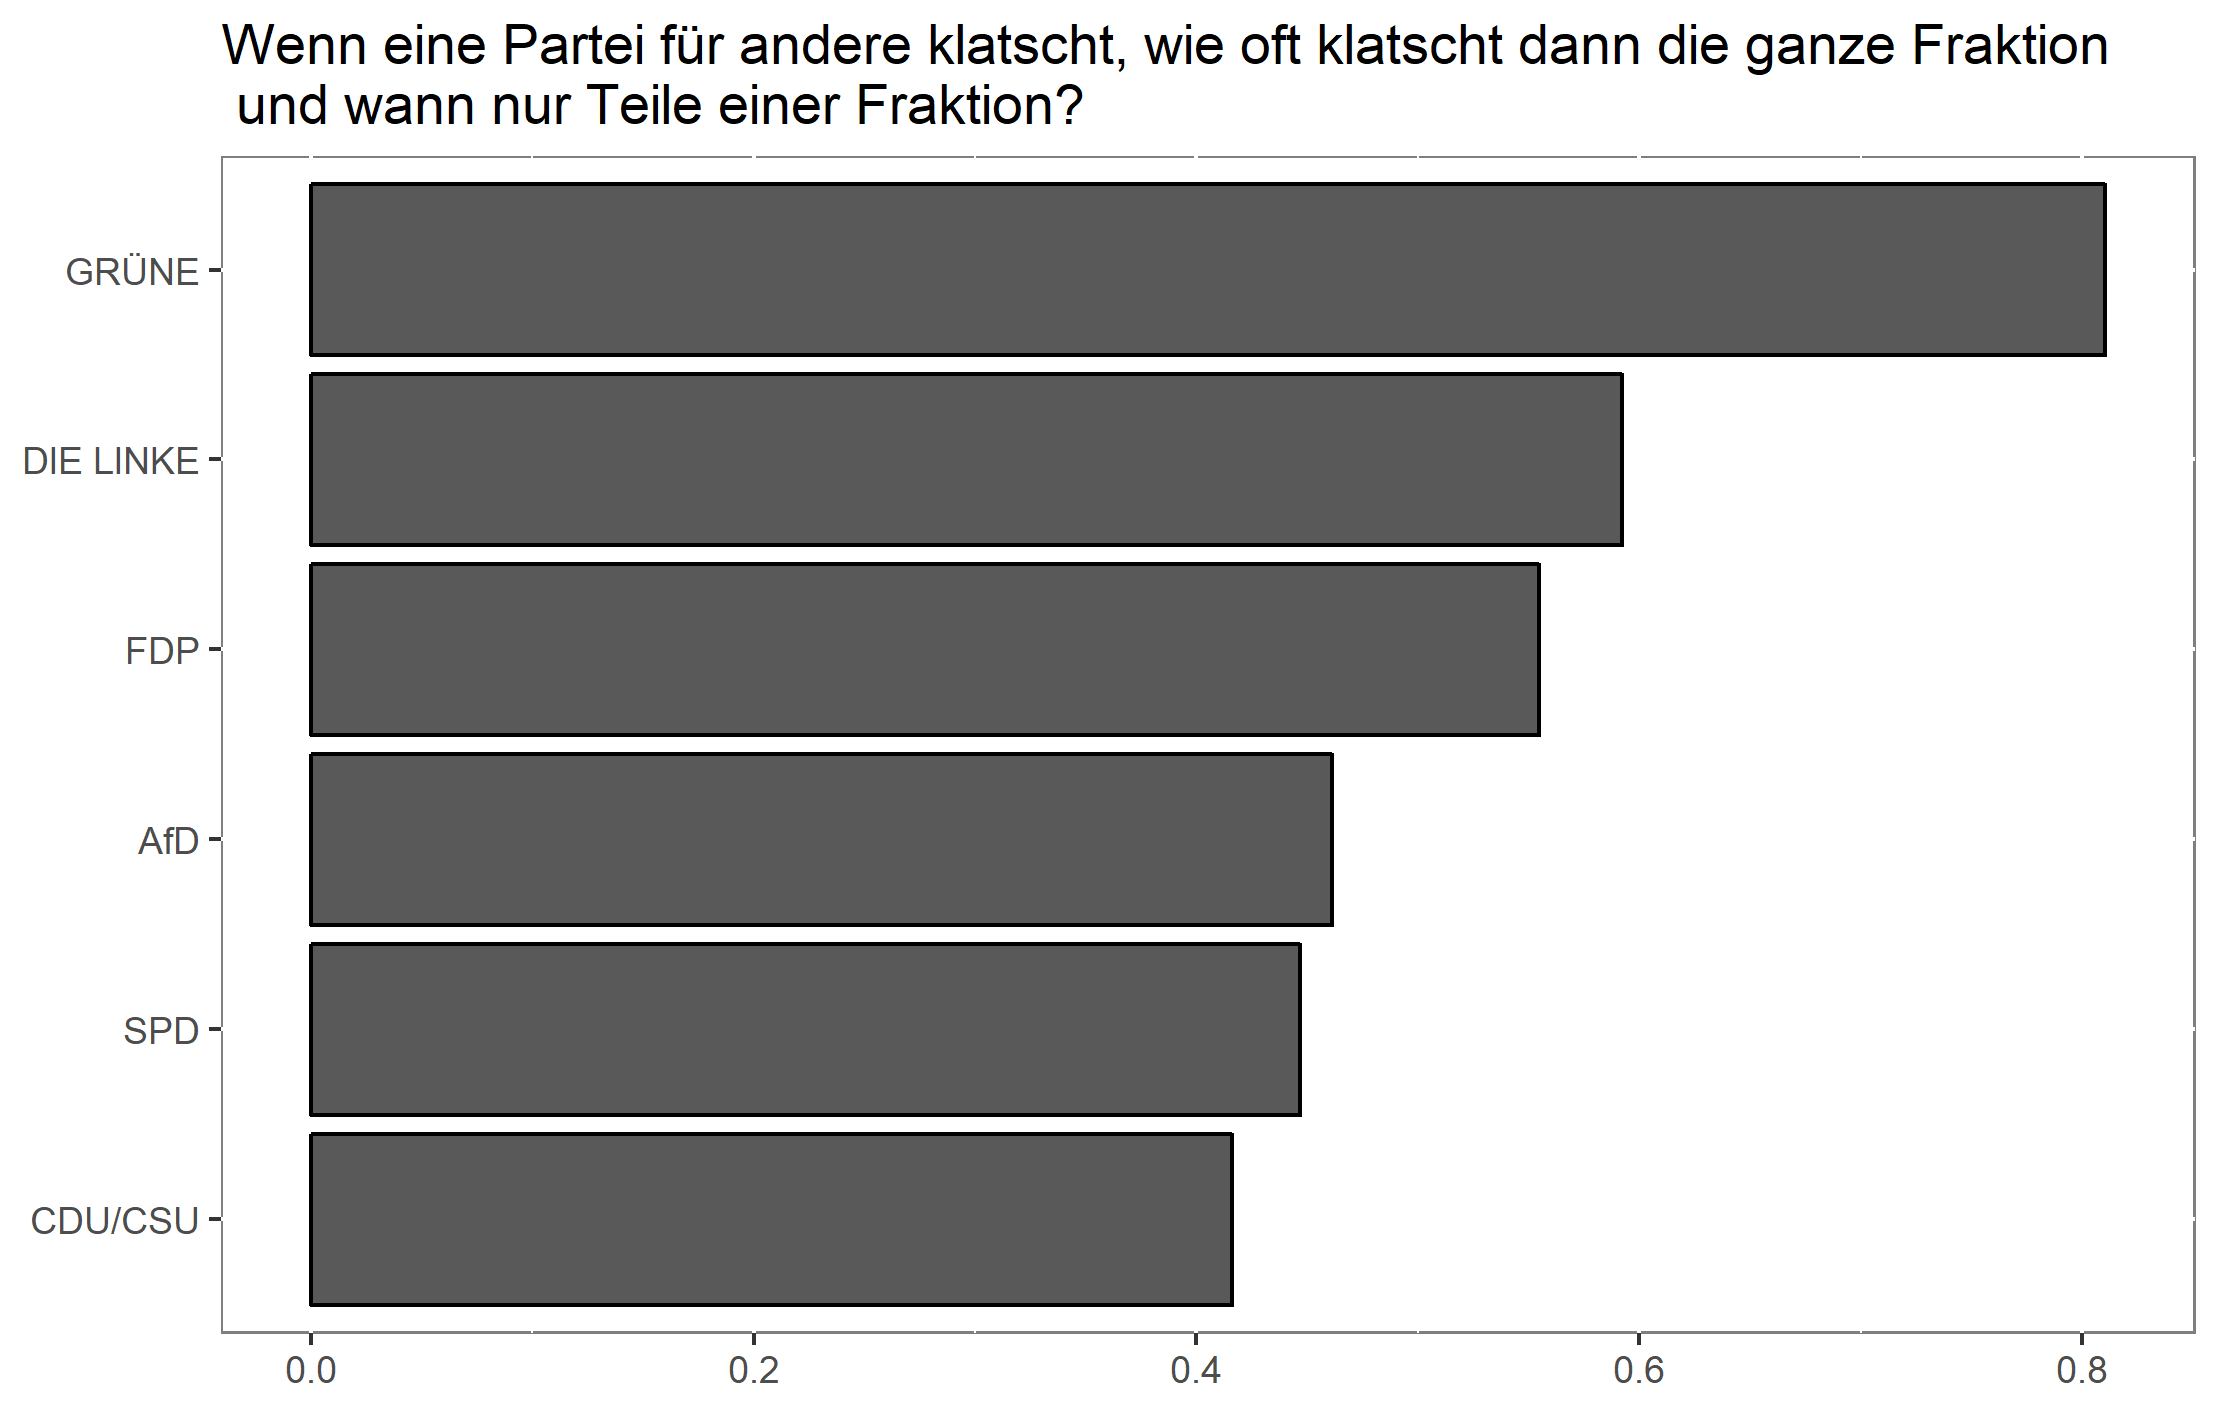
\includegraphics[width=0.5\linewidth]{Grafiken/Geschlossenheit17.png}\\

Es zeigt sich, dass weder die Hypothese bestätigt werden kann, dass es eine große Veränderung bezüglich der Geschlossenheit gegeben hat, noch, dass die AfD als Newcomer-Partei besonders geschlossen auftritt. Interessanter ist eher, dass sich der Fraktionsstreit der CDU mit der CSU deutlich in dem Ergebnis zeigt, dass die CDU/CSU plötzlich auf dem letzten Platz ist und in fast der Hälfte der Fälle nur einzelne Abgeordnete Klatschen und nicht die ganze Partei. 

\subsubsection{Isolierung in der Wortwahl} 
Die einzige Partei, die "Deutschland und deutsch" häufiger verwendet, als "Mensch" ist die AfD. Ein häufiges Nennen von bestimmten Worten zeigt die Bedeutung, die einem bestimmten Themenfeld beigemessen wird. xyx \\

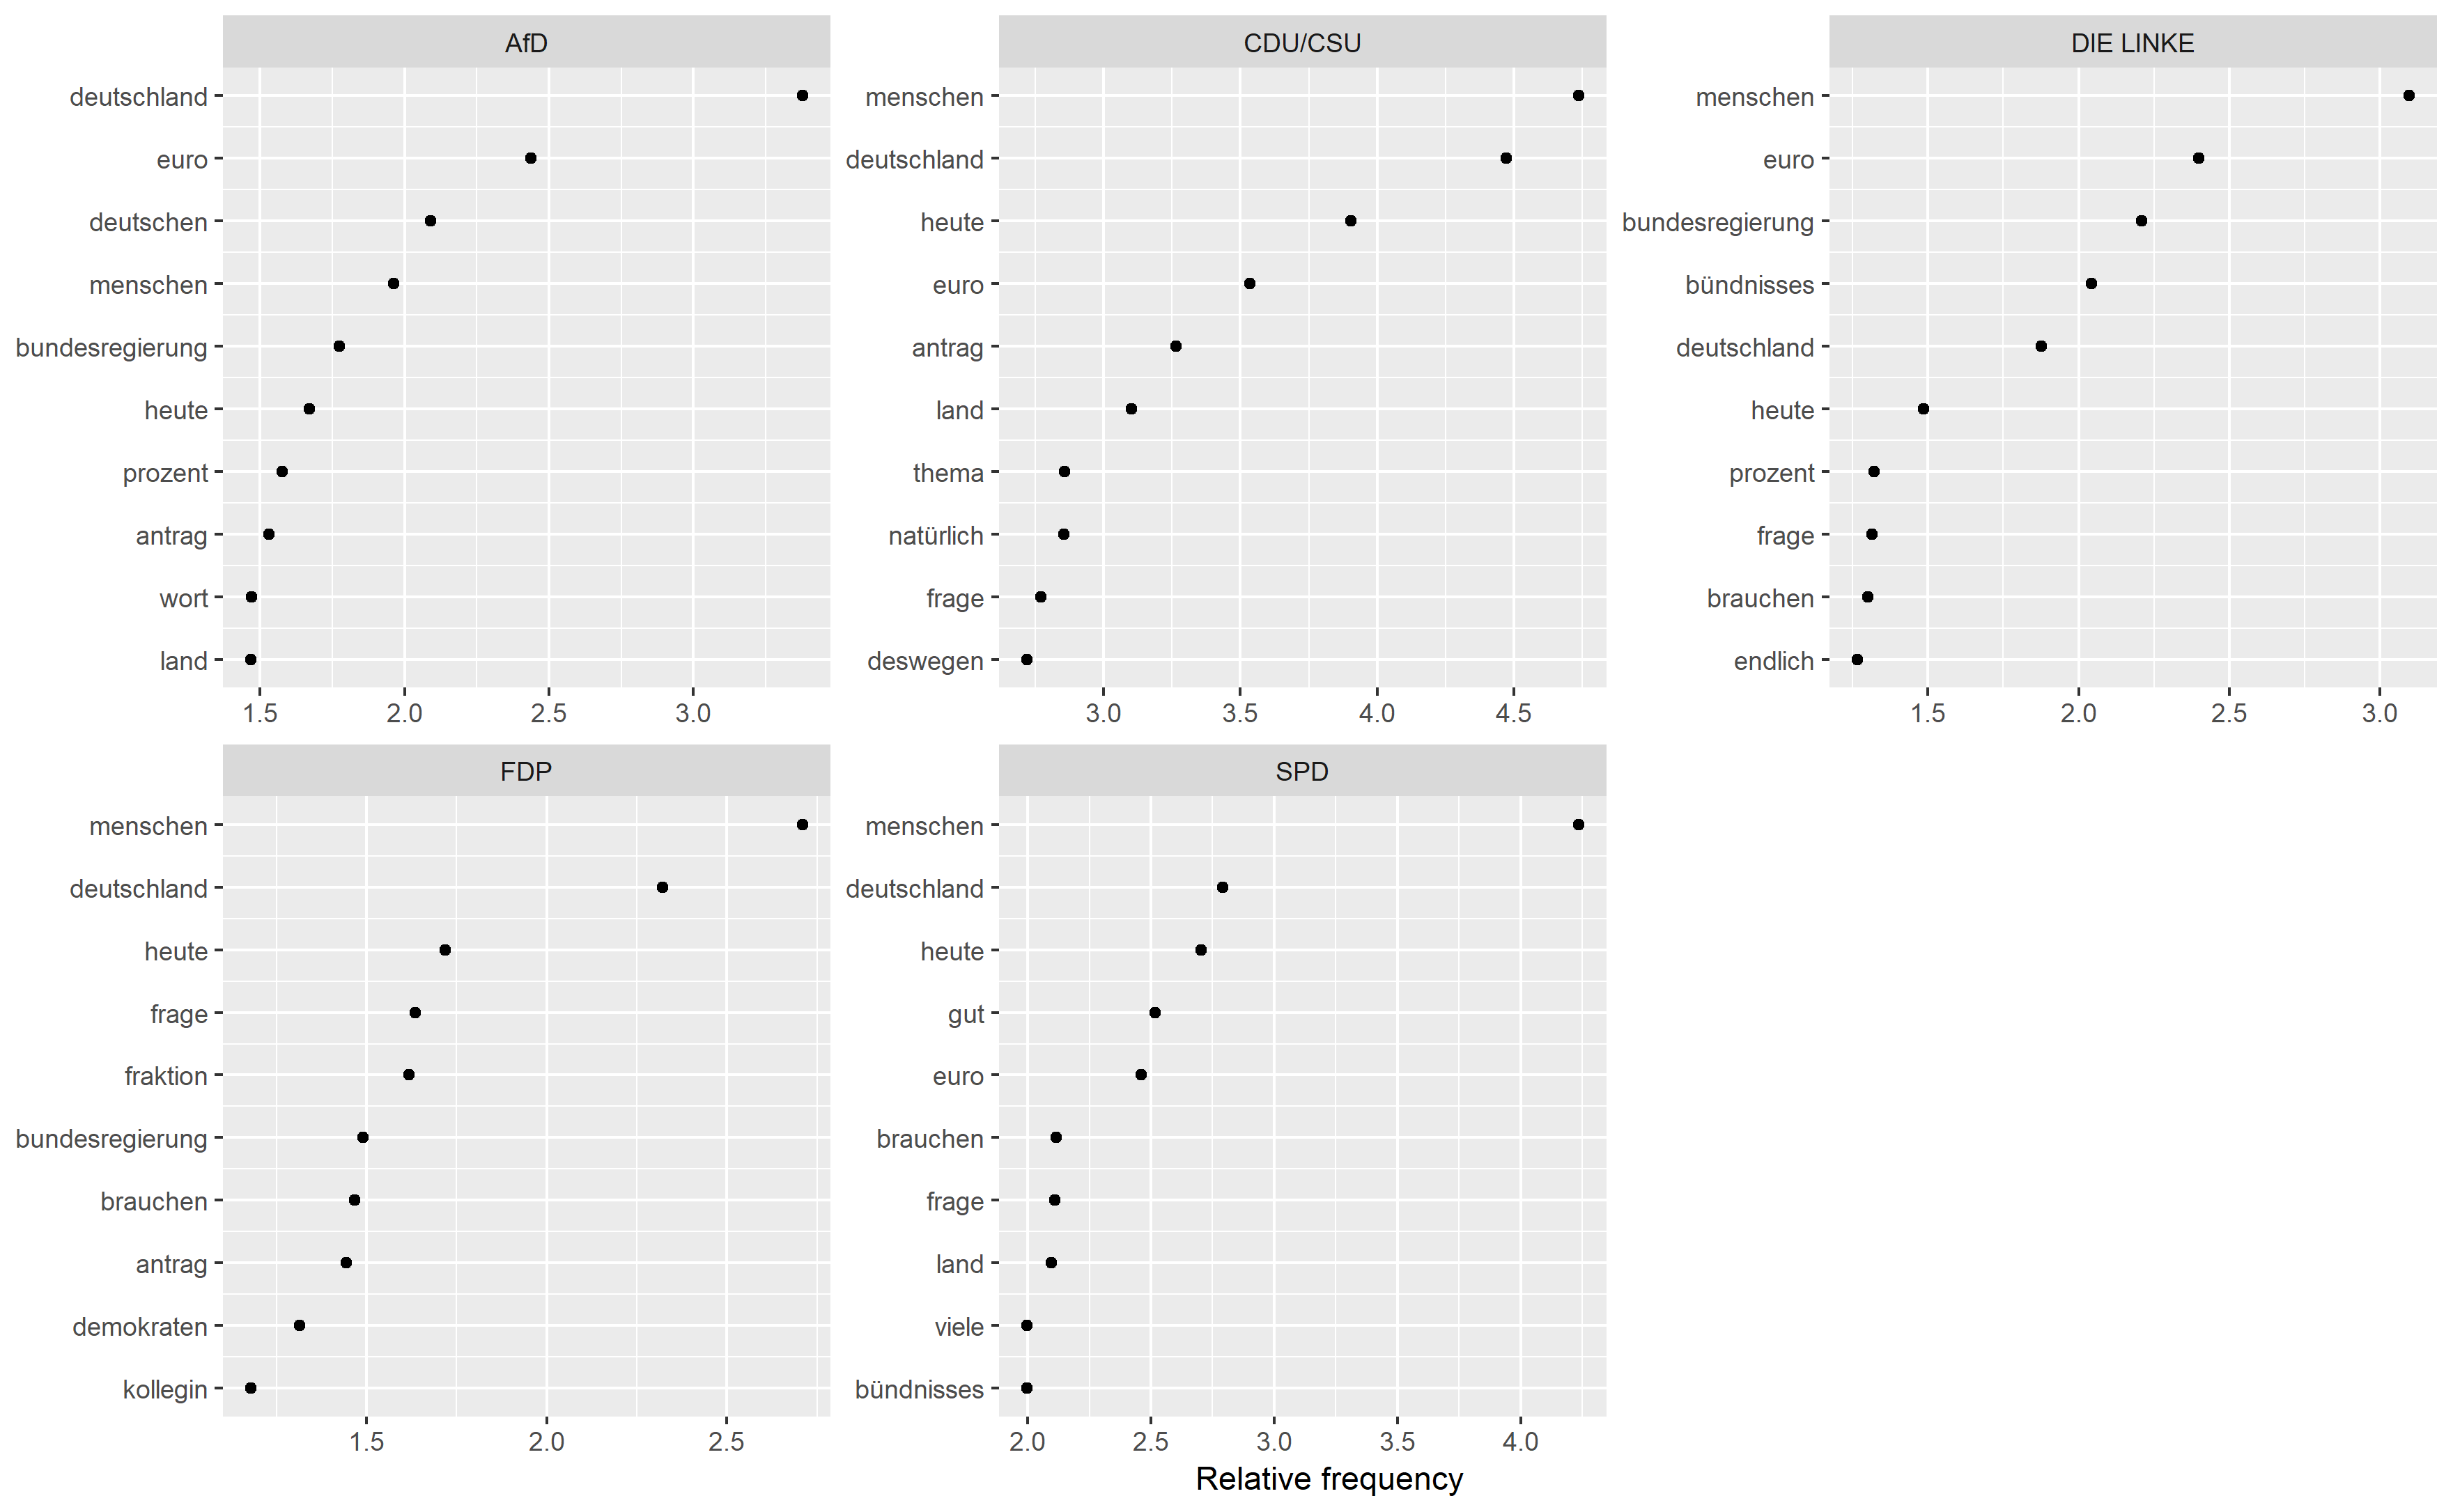
\includegraphics[width=\linewidth]{Grafiken/17_HäufigsteWörter.png}\\

\subsubsection{Negative Interaktionen}

"Lachen" wird vom stenografischen Dienst in Abgrenzung zur "Heiterkeit" als negative, Aktion beschrieben. Ebenso wird "Widerspruch" und "Zuruf", in Abgrenzung zu einem Kommentar, der sowohl positiv, als auch negativ sein kann, als negative Aktion beschrieben. 

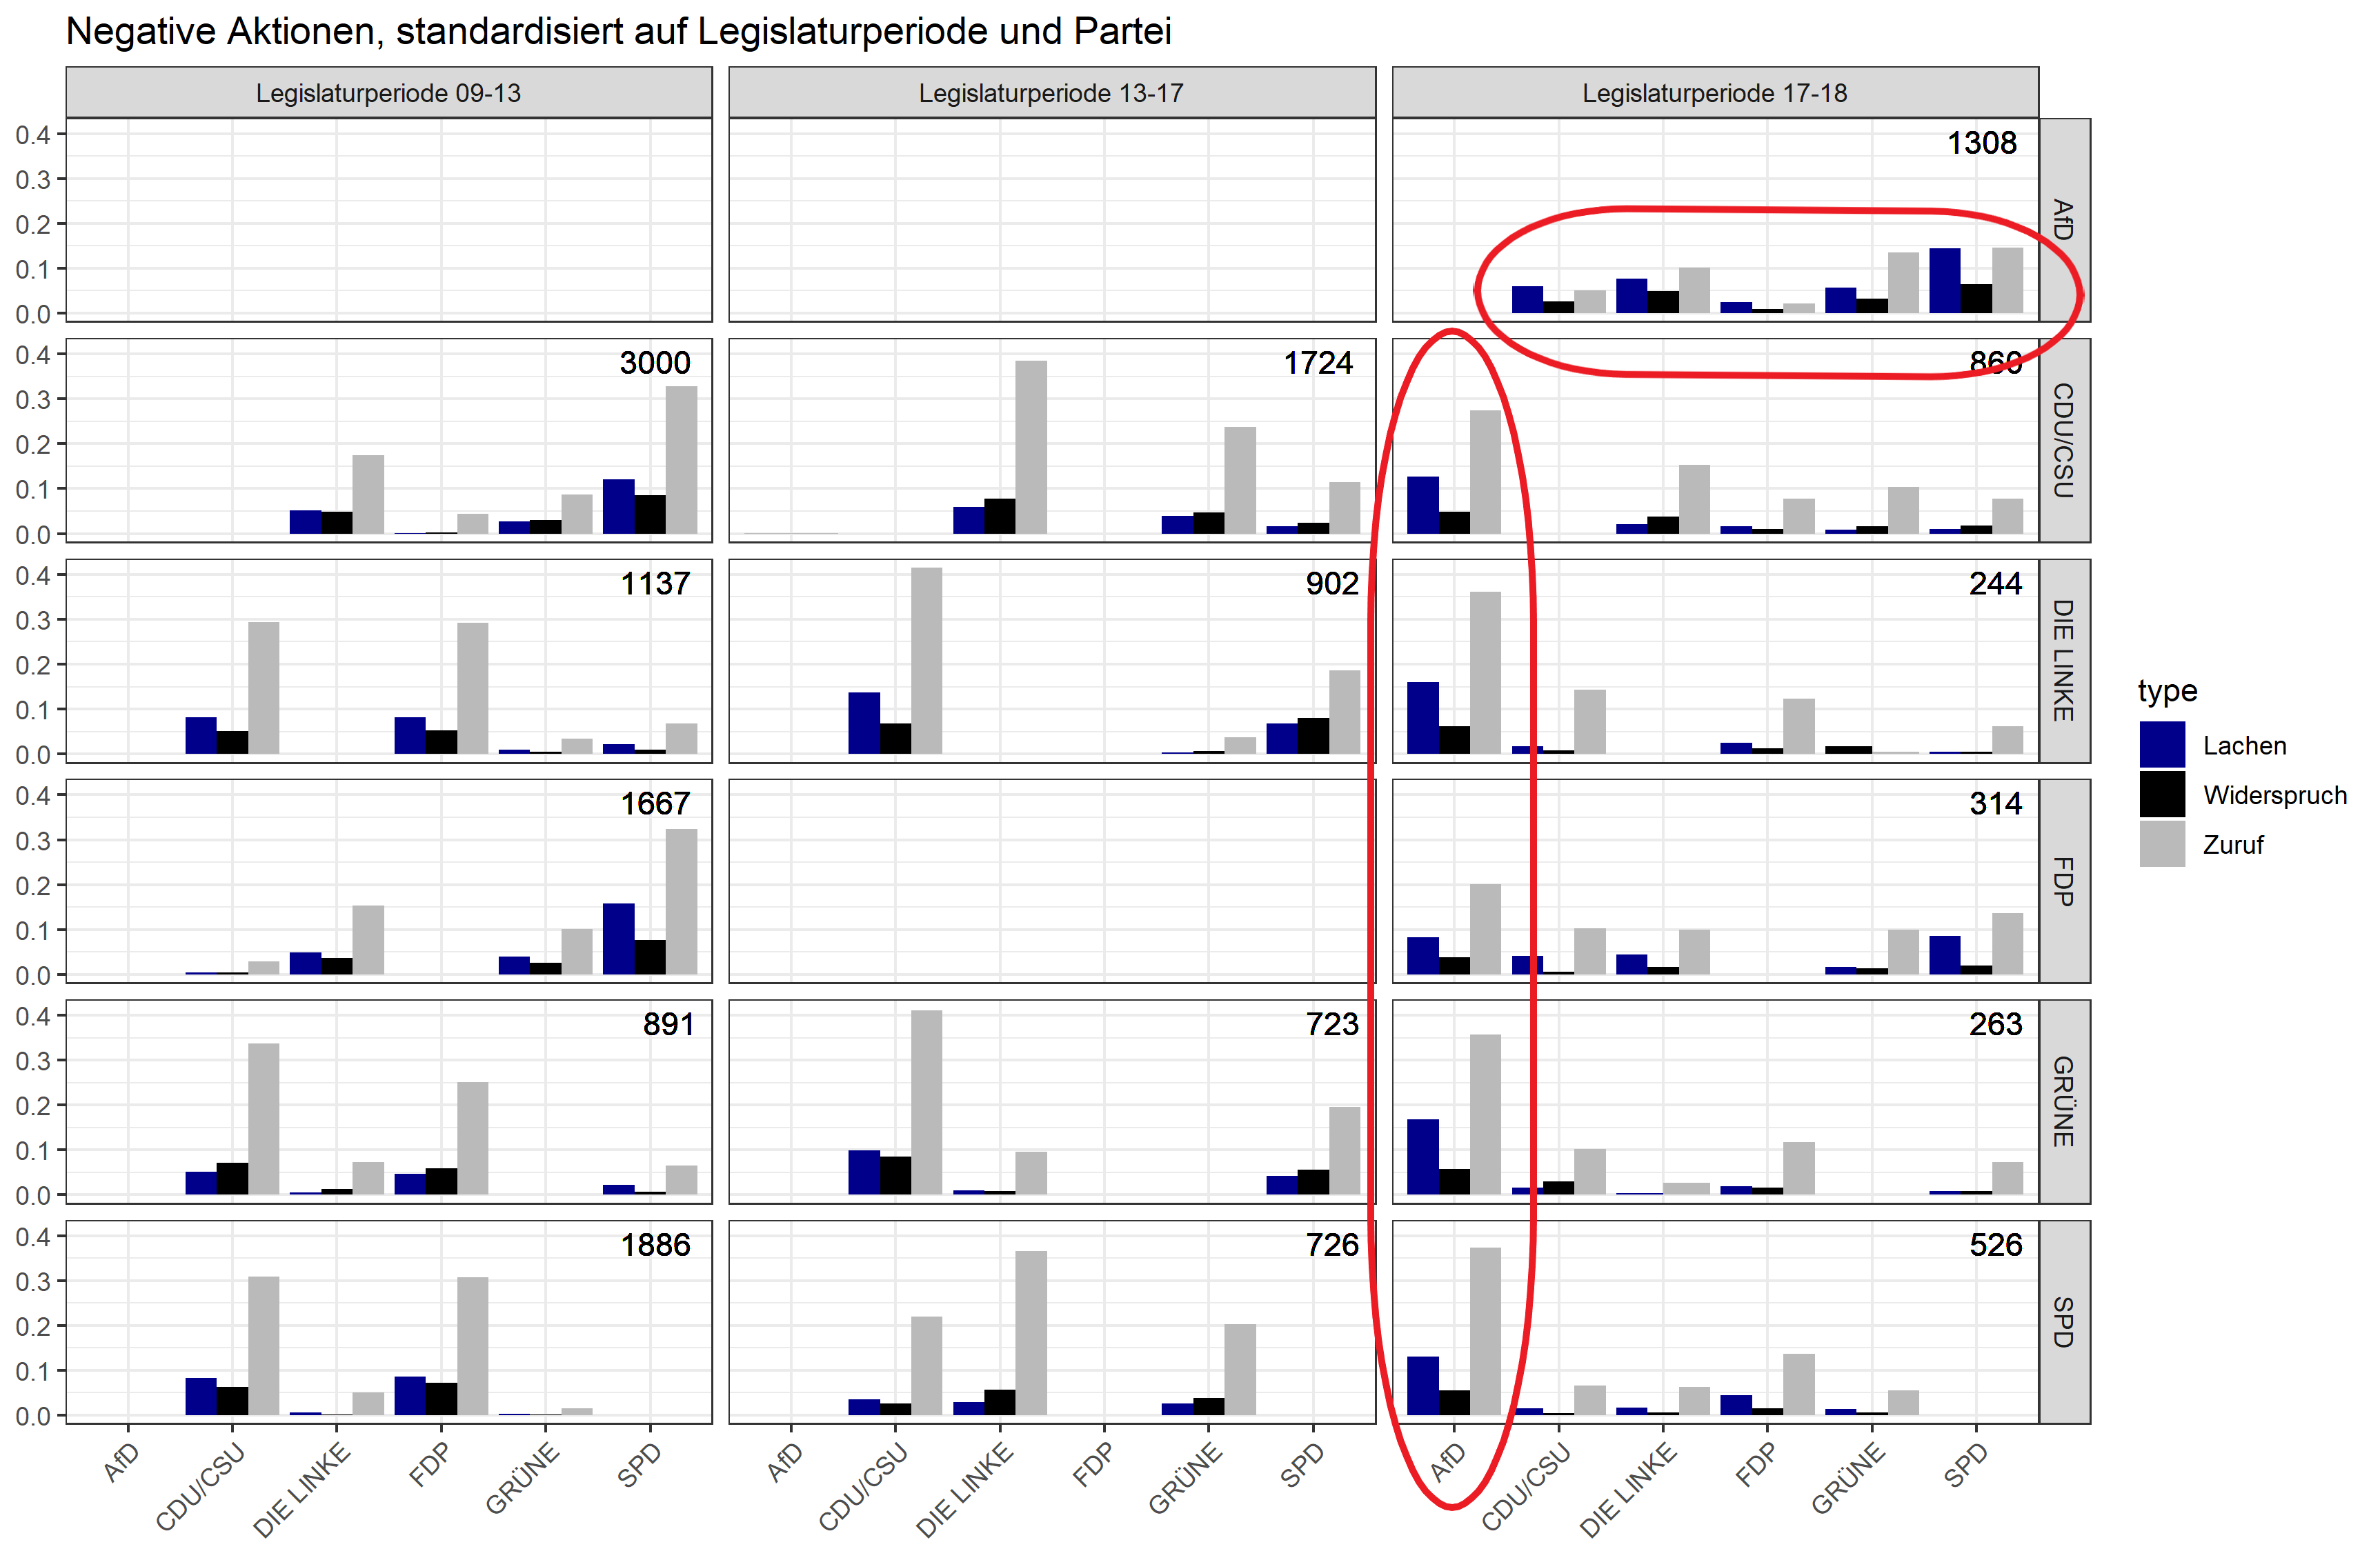
\includegraphics[width=\linewidth]{Grafiken/13_17negativ_perc_bunt.png}\\

Die Grafik zeigt, dass über die AfD am meisten gelacht, am meisten zugerufen und am meisten widersprochen wird. Die AfD ist aber auch die Partei, die die meisten negativen Interaktionen bei den anderen Parteien äußert. 



%\subsection{Sentiment}
%Die diktionär-basierte Sentimentanalyse hat keine nutzbaren Ergebnisse geliefert. Verwendet wurde das Wörterbuch der Uni- Leipzig (Quelle:), das gewichtete positive und negative Wörter enthält. \\
%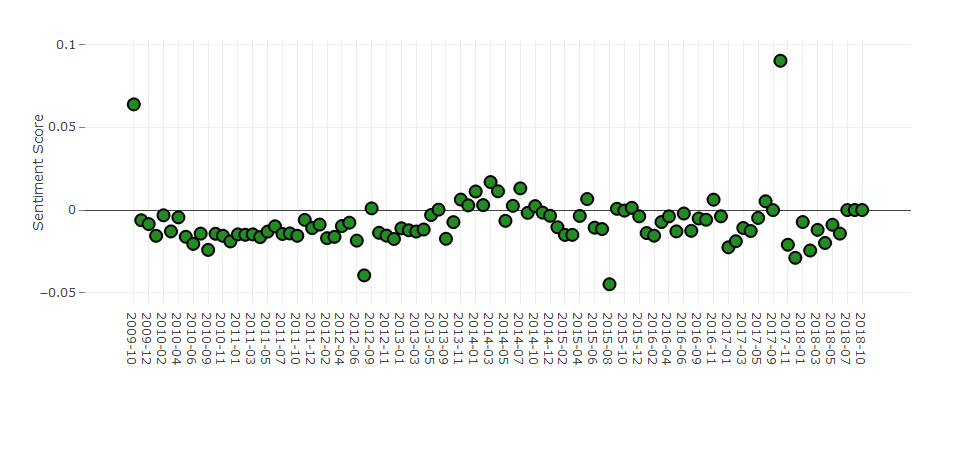
\includegraphics[width=\linewidth]{Grafiken/Sentimentscore.png}\\

